%% -*- coding:utf-8 -*-
\chapter{Transformational Grammar -- Minimalism}
\label{Abschnitt-MP}\label{chap-mp}\label{chapter-minimalism}\label{chapter-mp}

Like\is{Minimalist Program (MP)|(} the Government \& Binding framework that was introduced in the previous chapter, the Minimalist
framework was initiated by Noam Chomsky at the MIT in Boston. \citet{Chomsky93b-u,Chomsky95a-u}
argued that the problem of language evolution should be taken seriously and that the question of how
linguistic knowledge could become part of our genetic endowment should be answered. To that end he
suggested refocusing the theoretical developments towards models that have to make minimal
assumptions regarding the machinery that is needed for linguistic analyses and hence towards models
that assume less language specific innate knowledge.  

Like GB, Minimalism is wide-spread: theoreticians all over the world are working in this
framework, so the following list of researchers and institutions is necessarily
incomplete. \emph{Linguistic Inquiry} and \emph{Syntax} are journals that almost exclusively publish
Minimalist work and the reader is referred to these journals to get an idea about who is active in
this framework. 
%% There are hotspots at the MIT (David Pesetsky and Norvin Richards), in Maryland (Norbert
%% Hornstein), and at the University of Connecticut (Željko Bošković). Mamuro Saito is a Minimalist
%% working at the Nanzan University in Japan.
%% in Europa müsste man neben Rizzi und Cinque auch Cedric Boeckx und Marcel den Dicken nennen, David Adger, Peter Svenonius, Ian Roberts, Anders Holmberg 
The most prominent researchers in Germany are 
Artemis Alexiadou, Humboldt University Berlin; 
Günther \citet{Grewendorf2002a}, Frankfurt am Main; 
Joseph Bayer, Konstanz; 
and Gereon Müller, Leipzig.

While innovations like \xbart and the analysis of clause structure in GB are highly influential and
can be found in most of the other theories that are discussed in this book, this is less so for the
technical work done in the Minimalist framework. It is nevertheless useful to familiarize with the
technicalities since Minimalism is a framework in which a lot of work is done and understanding the basic machinery makes it possible to read empirically interesting
work in that framework.

%% The degree of formalization of Minimalist theories is not different from what is known from GB times (see
%% Sections~\ref{sec-formalization-gb}and ~\ref{sec-formalization-minimalism}) and as a result there are only few computerprocessable
%% implementations. Edward Stabler and colleagues developed so"=called \emph{Minimalist Grammars},
%% which are formalizations of some of Chomsky's and Kayne's ideas
%% \citep{Stabler2001a,Kobele2006a-u,GM2007a}. On Minimalist Grammars see also Section~\ref{sec-MG} of this
%% book. This formal work was also implemented by Stabler and others. In addition there
%% are implementations by Sandiway Fong \citep{FG2012a,Fong2014a} and \citet{NB2005a-u}. However, these implementations cover only some of
%% the aspects that are suggested in theoretical papers. They will be discussed in more detail in Section~\ref{sec-formalization-minimalism}.

While the GB literature of the 1980s and 1990s shared a lot of assumptions, there was an explosion of various
approaches in the Minimalist framework that is difficult to keep track of. The presentation that
follows is based on David Adger's textbook \citep{Adger2003a}.


\section{General remarks on the representational format}

The theories that are developed in the framework of the Minimalist Program build on the work done in
the GB framework. So a lot of things that were explained in the previous chapter can be taken over
to this chapter. However, there have been some changes in fundamental assumptions. The general
parametrized principles were dropped from the theory and instead the relevant distinctions live in
features. Languages differ in the values that certain features may have and in addition to this,
features may be strong\is{feature!strong} or weak\is{feature!weak} and feature strength\is{strength} is also a property that may vary from language
to language. Strong features make syntactic objects move to higher positions. The
reader is familiar with this feature"=driven movement already since it was a component of the movement"=based
analysis of the passive in Section~\ref{sec-passive-gb}. In the GB analysis of passive, the object
had to move to the specifier position of IP in order to receive case. Such movements that are due to
missing feature values are a key component in Minimalist proposals.


\subsection{Basic architecture}

Chomsky assumes that there are just two operations (rules) for combining linguistic objects:
External and Internal Merge. External Merge simply combines two elements like \emph{the} and
\emph{book} and results in a complex phrase. Internal Merge is used to account for movement of
constituents. It applies to one linguistic object and takes some part of this linguistic object and
adjoins it to the left of the respective object. The application of External Merge and Internal
Merge can apply in any order. For instance, two objects can be combined with External Merge and then
one of the combined items is moved to the left by applying Internal Merge. The resulting object can
be externally merged with another object and so on. As an example consider the NP in (\mex{1}):
\ea
the man who we know
\z
To derive this NP the verb \emph{know} is externally merged with its object \emph{who}. After
several intermediate merges that will be discussed below, \emph{know who} will be merged with
\emph{we} and finally the \emph{who} is moved to the left by Internal Merge, resulting in \emph{who
  we know}. This relative clause can be externally merged with \emph{man} and so on.

So, Minimalist theories differ from GB in not assuming a Deep Structure that is generated by some
\xbar grammar and a Surface Structure that is derived from the Deep Structure by \movea. Instead, it
is assumed that there is a phase in which External and Internal Merge (combination and movement)
apply in any order to derive a certain structure that is then said to be spelled out. It is said
that the structure is sent to the interfaces: the articulatory-perceptual system (AP) on the one hand and
the conceptual-intentional system (CI) on the other side. AP corresponds to the level of
Phonological Form (PF) and CI to the level of Logical Form (LF) in GB. The new architecture is
depicted in Figure~\vref{fig-architecture-minimalism}.
\begin{figure}
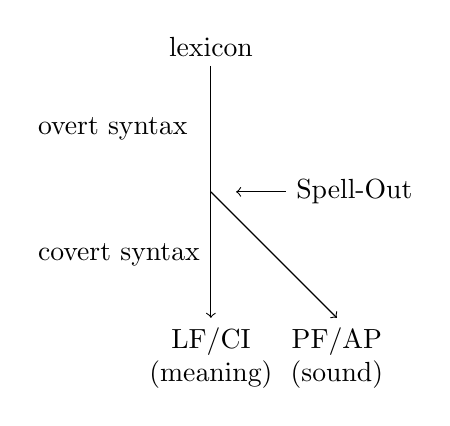
\begin{tikzpicture}[scale=.8]
%\draw (-2.9,-5.8) to[grid with coordinates] (2.7,-0.6);
\draw[->] (0,-1) node[anchor=south] {lexicon} --(0,-5) node[anchor=north, align=center] {LF/CI\\(meaning)};
\draw[->] (0,-3)--(2,-5) node[anchor=north,align=center] {PF/AP\\(sound)};
\draw[<-] (.4,-3)--(1.2,-3) node[anchor=west] {Spell-Out};
%\draw (0,-0.5) node {lexicon};
\draw (-2.9,-2) node[anchor=west] {overt syntax};
\draw (-2.9,-4) node[anchor=west] {covert syntax};
%\draw (0,-6.5) node[align=center] {LF/CI\\(meaning)};
%\draw (2,-5.5) node[align=center] {PF/AP\\(sound)};
\end{tikzpicture}
\caption{\label{fig-architecture-minimalism}Architecture assumed in Minimalist theories before the
  Phase model}
\end{figure}%
Overt syntax stands for syntactic operations that usually have a visible effect. After overt syntax
the syntactic object is sent off to the interfaces and some transformations may take place after
this Spell-Out point. Since such transformations do not affect pronunciation, this part of syntax is
called \emph{covert syntax}. Like in GB's LF, the covert syntax can be used to derive certain scope
readings. 

This architecture was later modified to allow Spell-Out at several points in the derivation. It is now
assumed that there are \emph{phases}\is{phase} in a derivation and that a completed phase is spelled out once it is
used in a combination with a head \citep{Chomsky2008a}. For instance, a subordinated sentence like \emph{that Peter comes} in (\mex{1}) is one
phase and is sent to the interfaces before the whole sentence is completed.\footnote{
  Andreas Pankau (p.\,c.\, 2015) pointed out to me that there is a fundamental problem with such a
  conception of phases, since if it is the case that only elements that are in a relation to a head
  are send off to the interface then the topmost phrase in a derivation would never be sent to the interfaces, since it does not depend on any head.
}

\ea
He believes that Peter comes.
\z
There are different proposals as to what categories form complete phases. Since the concept of
phases is not important for the following introduction, I will ignore this concept in the following. See Section~\ref{sec-dtc} on the psycholinguistic plausibility of phases in
particular and the Minimalist architecture in general. 

\subsection{Valence, feature checking, and agreement}
\label{sec-features-minimalism}

The basic mechanism in Minimalist theories is feature checking.\is{feature!checking} For instance, the noun
\emph{letters} may have a P feature, which means that it has to combine with a PP in order to form a complete phrase.
\ea
letters to Peter
\z
It is assumed that there are interpretable and uninterpretable features. An example of an
interpretable feature is the number feature of nouns. The singular/plural distinction is
semantically relevant. The category features for part of speech information are purely syntactic and
hence cannot be interpreted semantically. Minimalism assumes that all uninterpretable features have
to be used up during the derivation of a complex linguistic object. This process of eating up the
features is called \emph{checking}. As an example, let us consider the noun \emph{letters} again. The
analysis of (\mex{0}) is depicted in Figure~\vref{fig-letters-to-peter-minimalism}.
\begin{figure}
\centering
\begin{forest}
baseline
[N 
  [\emph{letters} {[N, pl, \st{\textit{u}P}]}]
  [P
    [\emph{to} {[P, \st{\textit{u}N}]}]
    [\emph{Peter} {[N]}]]]
\end{forest}
\caption{\label{fig-letters-to-peter-minimalism}Valence representation via uninterpretable features}
\end{figure}%
The fact that the P feature of \emph{letters} is uninterpretable is represented by the little
\emph{u} in front of the P. The uninterpretable P feature of \emph{letters} can be checked against
the P feature of \emph{to Peter}. All checked features are said to delete\is{feature!deletion} automatically. The
deletion is marked by striking the features out in the figures. Strings like (\mex{1}) are ruled out as complete derivations since
the N feature of P is not checked. This situation is shown in Figure~\vref{fig-letters-to-minimalism}.
\ea[*]{
letters to
}
\z
\begin{figure}
\centering
\begin{forest}
baseline
[N 
  [\emph{letters} {[N, pl, \st{\textit{u}P}]}]
  [\emph{to} {[P, \textit{u}N]}]]
\end{forest}
\caption{\label{fig-letters-to-minimalism}Illegitimate syntactic object due to an uninterpretable feature}
\end{figure}%
If this structure would be used in a larger structure that is spelled out, the derivation would
\emph{crash} since the conceptual system could not make sense of the N feature that is still present
at the P node.

Selectional features are atomic, that is, the preposition cannot select an NP[\type{acc}] as in GB
and the other theories in this book unless NP[\type{acc}] is assumed to be atomic. Therefore, an
additional mechanism is assumed that can check other features in addition to selectional
features. This mechanism is called \emph{Agree}\is{Agree|(}.
\eal
\ex[*]{
letters to he
}
\ex[]{
letters to him
}
\zl
The analysis of (\mex{0}b) is shown in Figure~\vref{fig-letters-to-him-minimalism}.
\begin{figure}
\centering
\begin{forest}
baseline
[N 
  [\emph{letters} {[N, pl, \st{\textit{u}P}]}]
  [P
    [\emph{to} {[P, \st{\textit{u}N}, \st{acc}]}]
    [\emph{him} {[N, \st{acc}]}]]]
\end{forest}
\caption{\label{fig-letters-to-him-minimalism}Feature checking via Agree}
\end{figure}%
There is an interesting difference between the checking of selectional features and the checking of
features via Agree. The features that are checked via Agree do not have to be at the top node of the
object that is combined with a head. This will play a role later in the analysis of the passive and
local reordering.%
\is{Agree|)}

\subsection{Phrase structure and \xbart}

The projections of \xbar structures were given in Figure~\ref{Abb-GB-Min-Max} on
page~\pageref{Abb-GB-Min-Max}. According to early versions of the \xbart, there could be arbitrarily
many complements that were combined with \xzero to form an \xbar. Arbitrarily many adjuncts could
attach to \xbar and then at most one specifier could be combined with the \xbar yielding an
XP. Minimalist theories assume binary branching and hence there is at most one
complement, which is the first-merged item. Furthermore, it is not assumed that there is a unique
specifier position. Chomsky rather assumes that all items that are not complements are
specifiers. That is, he distinguishes between first-merged (complements) and later-merged items (specifiers). Figure~\vref{fig-head-comp-spec} shows an example with two specifiers.
\begin{figure}
\centering
\begin{forest}
%where n children=0{}{},
%sn edges
%for tree={parent anchor=south, child anchor=north,align=center,base=bottom}
[XP
  [specifier]
  [\xbar
    [specifier]
    [\xbar
      [complement] [X] ] ] ]
\end{forest}
\caption{\label{fig-head-comp-spec}Complements and specifiers in Minimalist theories}
\end{figure}%
It is also possible to have just a complement and no specifier or to have one or three
specifiers. What structures are ultimately licensed depends on the features of the items that are
involved in the Merge operations. Whether a phrasal projection counts as an \xbar or an XP depends
on whether the phrase is used as a complement or specifier of another head or whether it is used as
head in further Merge operations. If a phrase is used as specifier or complement its status is fixed
to be a phrase (XP), otherwise the projectional status of resulting phrases is left
underspecified. Lexical head daughters in Merge operations have the category X and complex head
daughters in Merge operations have the category \xbar. This solves the problem that standard \xbar
theoretic approaches had with pronouns and proper names: a lot of unary branching structure had to
be assumed (See left picture in Figure~\ref{Abb-GB-Min-Max}). This is not necessary any longer in
current Minimalist theories.\footnote{
  For problems with this approach see \citew[Chapter~2.1]{Brosziewski2003a-u}. 
%% Das ist zu viel hier.
%% It is interesting to
%%   note that these problems do not apply to Categorial Grammar and HPSG, which use techniques for avoiding unary branchings
%%   that are similar to the ones suggested by  
}


\subsection{Little \textit{v}}
\label{sec-little-v}

In\is{category!functional!v@\textit{v}|(} Section~\ref{sec-passive-gb}, I used \xbar structures in which a ditransitive verb was combined
with its accusative object to form a \vbar, which was then combined with the dative object to form a
further \vbar. Such binary branching structures and also flat structures in which both objects are
combined with the verb to form a \vbar are rejected by many practitioners of GB and Minimalism since
the branching does not correspond to branchings that would be desired for phenomena like the binding
of reflexives and negative polarity items. A binding in which \emph{Benjamin} binds \emph{himself}
in (\mex{1}a) is impossible:
\eal
\ex[*]{
Emily showed himself Benjamin in the mirror.
}
\ex[]{
Peter showed himself Benjamin in the mirror.
}
\zl
What is required for the analysis of Binding and NPI phenomena in theories that analyze these
phenomena in terms of tree configurations is that the reflexive pronoun is ``higher'' in the tree than
the proper name \emph{Benjamin}. More precisely, the reflexive pronoun \emph{himself} has to
c-command \emph{Benjamin}. c-command is defined as follows \citep[\page 117]{Adger2003a}:\footnote{
  c-command also plays a prominent role in GB. In fact, one part of Government \& Binding is the
  Binding Theory, which was not discussed in the previous chapter since binding phenomena do not
  play a role in this book.
}
\ea
A node A c-commands B if, and only if A's sister either:\\
\begin{tabular}[t]{@{}l@{~}l@{}}
a. & is B, or\\
b. & contains B
\end{tabular}
\z

In the trees to the left and in the middle of Figure~\vref{fig-ditransitives-options} the c-command
relations are not as desired: in the left-most tree both NPs c-command each other and in the middle
one \emph{Benjamin} c-commands \emph{himself} rather than the other way round.
\begin{figure}
\begin{forest}
baseline
[\vbar
 [\textit{show}]
 [\textit{himself}]
 [\textit{Benjamin}]]
\end{forest}
\hfill
\begin{forest}
baseline
[\vbar
   [\vbar
     [\textit{show}]
     [\textit{himself}] ]
 [\textit{Benjamin}]]
\end{forest}
\hfill\hfill
\begin{forest}
baseline
[\littlevbar
 [\textit{show}]
 [VP
   [\textit{himself}]
   [\vbar
    [V]
    [\textit{Benjamin}]]]]
\end{forest}
\caption{\label{fig-ditransitives-options}Three possible analyses of ditransitives}
\end{figure}%
Hence it is assumed that the structures at the left and in the middle are inappropriate and that
there is some additional structure involving the category \textit{v}, which is called \emph{little v}
\citep[Section~4.4]{Adger2003a}. The sister of \emph{himself} is \vbar and \vbar contains
\emph{Benjamin}, hence \emph{himself} c-commands \emph{Benjamin}. Since the sister of
\emph{Benjamin} is V and V neither is nor contains \emph{himself}, \emph{Benjamin} does not
c-command \emph{himself}. 

The analysis of ditransitives involving an additional verbal head goes back to
\citet{Larson88a}. \citet[\page 70]{HK93a-u} assume that this verbal head contributes a causative
semantics.
%% \todostefan{Andrew McIntyre: the idea of causative light verbs was not used by Larson 1988. (I think
%%   it started in Hale \& Keyser 1993.) Larson also didn't use the term 'little v' (I am not sure, but
%%   I think that term was introduced in Chomsky's black book).} 
The structure in Figure~\ref{fig-ditransitives-little-v} is derived by assuming that the verb \emph{show} starts out
in the V position and then moves to the \textit{v} position. \emph{show} is assumed to mean
\emph{see} and in the position of \littlev it picks up the causative meaning, which results in a
\relation{cause-see} meaning \citep[\page 133]{Adger2003a}. 
\begin{figure}
\centering
\begin{forest}
baseline
[\vP
  [\textit{Peter}]
  [\littlevbar
   [\textit{v} $+$ \textit{show}]
   [VP
     [\textit{himself}]
     [\vbar
      [\phonliste{ show } {[V]}]
      [\textit{Benjamin}]]]]]
\end{forest}
\caption{\label{fig-ditransitives-little-v}Analysis of ditransitives involving movement to \littlev}
\end{figure}%

While the verb shell analysis with an empty verbal head was originally invented by \citet{Larson88a}
for the analysis of ditransitive verbs, it is now also used for the analysis of strictly transitive
and even intransitive verbs.

\citet[Section~4.5]{Adger2003a} argues that semantic roles are assigned uniformly in certain tree
configurations:
\eal
\ex NP daughter of \vP $\to$ interpreted as agent
\ex NP daughter of VP $\to$ interpreted as theme
\ex PP daughter of \littlevbar $\to$ interpreted as goal
\zl
Adger assumes that such uniformly assigned semantic roles help in the process of language
acquisition\is{language acquisition} and from this, it follows that \littlev should also play a role in the analysis of
examples with strictly transitive and intransitive verbs. The
Figures~\ref{fig-transitives-little-v} and~\ref{fig-intransitives-little-v} show the analysis of
sentences containing the verbs \emph{burn} and \emph{laugh}, respectively.\footnote{
  If all intransitive verbs of this type are supposed to have agents as subjects, a very broad
  conception of agent has to be assumed that also subsumes the subject of verbs like
  \emph{sleep}. Usually sleeping is not an activity that is performed intentionally.
}
\begin{figure}
\centering
\begin{forest}
baseline
[\vP
  [Agent]
  [\littlevbar~{[\st{\textit{u}D}]}
   [\textit{v}]
   [VP
      [\textit{burn} {[V, \st{\textit{u}D}]}]
      [Theme]]]]]
\end{forest}
\caption{\label{fig-transitives-little-v}Analysis of strictly transitives involving \littlev}
\end{figure}%

\begin{figure}
\centering
\begin{forest}
baseline
[\vP
  [Agent]
  [\littlevbar~{[\st{\textit{u}D}]}
   [\textit{v} ]
   [ \textit{laugh} {[V]} ]]]
\end{forest}
\caption{\label{fig-intransitives-little-v}Analysis of intransitives involving \littlev}
\end{figure}%
%
\citet[\page 164]{Adger2003a} assumes that intransitive and transitive verbs move from V to \littlev
as well. This will be reflected in the following figures.%
\is{category!functional!v@\textit{v}|)}

\subsection{CP, TP, \vP, VP}
\label{sec-CP-TP-vP-VP}


Section~\ref{sec-GB-CP-IP-System-English} dealt with the CP/IP system in GB. In the course of the
development of Minimalism, the Inflectional Phrase was split into several functional projections \citep{Chomsky89a-u}
% AgrS, TP, Neg, AgrO
of which only the Tense\is{category!functional!Tense} Phrase is assumed in current
Minimalist analyses. So, the TP of Minimalism corresponds to IP in the GB analysis. Apart from this
change, the core ideas of the CP/IP analysis have been transferred to
the Minimalist analysis of English. This subsection will first discuss 
special features that are assumed to trigger movement (Subsection~\ref{sec-epp-features}) and then 
case assignment (Subsection~\ref{sec-case-mp}).




\subsubsection{Features as triggers for movement: The EPP feature on T}
\label{sec-epp-features}


In GB approaches, the modals and auxiliaries were analyzed as members of the
category I and the subjects as specifiers of IP. In the previous section, I showed how subjects are
analyzed as specifiers of \vP. Now, if one assumes that a modal verb combines with such a \vP, the
subject follows the modal, which does not correspond to the order that is observable in English. This
problem is solved by assuming a strong uninterpretable D feature at T. Since the feature is strong,
a suitable D has to move to the specifier of T and check the D
locally. Figure~\vref{fig-Anna-will-read-the-book-minimalism} shows the TP that plays a role in the
analysis of (\mex{1}):
\ea
Anna will read the book.
\z
\begin{figure}
\centering
\begin{forest}
baseline
[TP
 [\textit{Anna} {[D]}]
 [\tbar{[\st{\textit{u}D*}]}
   [\textit{will} T{[pres]}]
   [\vP
     [\phonliste{ Anna }]
     [\littlevbar~{[\st{\textit{u}D}]}
       [\textit{v}
         [\textit{read}] [\textit{v}]]
       [VP
         [\phonliste{ read } {[V, \st{\textit{u}D}]}]
         [DP [\textit{the book}, triangle]]]]]]]
\end{forest}
\caption{\label{fig-Anna-will-read-the-book-minimalism}Analysis of \emph{Anna will read the book.}
  involving a modal and movement of the subject from \textit{v} to T}
\end{figure}%
The DP \emph{the book} is the object of \emph{read} and checks the D feature of
\emph{read}. \littlev selects for the subject \emph{Anna}. Since T has a strong D feature (marked by
an asterisk `*'\is{*}), \emph{Anna} must not remain inside of the \vP but moves on to the specifier position of TP.


Full sentences are CPs. For the analysis of (\mex{0}), an empty C head is assumed that is combined
with the TP. The empty C contributes a clause type feature Decl. The full analysis of (\mex{0}) is
shown in Figure~\ref{fig-Anna-will-read-the-book-minimalism-CP}.
\begin{figure}
\centering
\begin{forest}
baseline
[CP
 [C{[Decl]}]
 [TP
 [\textit{Anna} {[D]}]
 [\tbar{[\st{\textit{u}D*}]}
   [\textit{will} T{[pres]}]
   [\vP
     [\phonliste{ Anna }]
     [\littlevbar~{[\st{\textit{u}D}]}
       [\textit{v}
         [\textit{read}] [\textit{v}]]
       [VP
         [\phonliste{ read } {[V, \st{\textit{u}D}]}]
         [DP [\textit{the book}, triangle]]]]]]]]
\end{forest}
\caption{\label{fig-Anna-will-read-the-book-minimalism-CP}Analysis of \emph{Anna will read the book.}
  as CP with an empty C with the clause-type feature Decl}
\end{figure}%

%%
%% This is revised later to use an empty wh operator.
%% Too complicated.
%%
%% The analysis of the question in (\mex{1}) involves a strong Q feature for the sentence
%% type question.
%% \ea
%% Will Anna read the newspaper?
%% \z
%% The analysis is shown in Figure~\vref{fig-Will-Anna-read-the-newspaper-minimalism}.
%% \begin{figure}
%% \centering
%% \begin{forest}
%% baseline
%% [CP
%%    [C
%%      [\textit{will} T{[\st{Q*}]}]
%%      [C{[Q]}] ]
%%    [TP
%%    [\textit{Anna} {[D]}]
%%    [\tbar{[\st{\textit{u}D*}]}
%%      [\phonliste{ will } {[T]}]
%%      [\vP
%%        [\phonliste{ Anna }]
%%        [\littlevbar
%%          [\textit{v}]
%%          [VP
%%            [\textit{read} {[V, \textit{u}D]}]
%%            [DP [\textit{the newpaper},triangle]]]]]]]]]
%% \end{forest}
%% \caption{\label{fig-Will-Anna-read-the-newspaper-minimalism}Analysis of \emph{Will Anna read the
%%     news paper?}   with an empty C with a strong Q feature for encoding the clause type}
%% \end{figure}%
%% The analysis is parallel to the analysis of the declarative clause except that the modal verb moves
%% to C in order to check the strong Q feature locally.

The analysis of the question in (\mex{1}) involves an unvalued clause-type feature on T for the sentence type
\emph{question}. 
\ea
What will Anna read?
\z
The empty complementizer C has a Q feature that can value the clause-type feature on
T. Since clause-type features on T that have the value Q are stipulated to be strong, the T element
has to move to C to check the feature locally. In addition, the \emph{wh} element is moved. This
movement is enforced by a strong wh feature on C. The analysis of (\mex{0})
is given in Figure~\vref{fig-What-will-Anna-read-minimalism}.
\begin{figure}
\centering
\begin{forest}
baseline
[CP
 [\textit{what} {[D, wh]}]
 [\cbar{[\st{\textit{u}wh*}]}
   [C
     [\textit{will} T{[\st{Q*}]}]
     [C{[Q]}] ]
   [TP
   [\textit{Anna} {[D]}]
   [\tbar{[\st{\textit{u}D*}]}
     [\phonliste{ will } {[T]}]
     [\vP
       [\phonliste{ Anna }]
       [\littlevbar~{[\st{\textit{u}D}]}
         [\textit{v}
           [\textit{read}] [\textit{v}]]
         [VP
           [\phonliste{ read } {[V, \st{\textit{u}D}]}]
           [\phonliste{what}]]]]]]]]
\end{forest}
\caption{\label{fig-What-will-Anna-read-minimalism}Analysis of \emph{What will Anna read?}
  with an empty C with a strong wh feature}
\end{figure}%


%% \ea
%% C > T > (Neg) > (Perf) > (Prog) > (Pass) > \textit{v} > V
%% \z

\subsubsection{Case assignment}
\label{sec-case-mp}

In the GB analysis that was presented in Chapter~\ref{chap-gb}, nominative was assigned by (finite)
I and the other cases by the verb (see Section~\ref{sec-case-assignment}). The assignment of
nominative is taken over to Minimalist analyses, so it is assumed
that nominative is assigned by (finite) T. However, in the Minimalist theory under consideration, there
is not a single verb projection, but there are two verbal projections: \vP and VP. Now, one could
assume that V assigns accusative to its complement or that \textit{v} assigns accusative to the
complement of the verb it dominates. \citet[Section~6.3.2, Section~6.4]{Adger2003a} assumes the latter
approach, since it is compatible with the analysis of so-called unaccusative verbs and the passive. Figure~\vref{fig-Anna-reads-the-book-minimalism-TP} shows the TP for (\mex{1}):
\ea
Anna reads the book.
\z
\begin{figure}
\centering
\begin{forest}
baseline
[TP
 [\textit{Anna} {[D, \st{nom}]}]
 [\tbar{[\st{\textit{u}D*}, \st{nom}]}
   [T{[pres]}]
   [\vP
     [\phonliste{ Anna }]
     [\littlevbar~{[\st{\textit{u}D}]}
       [\textit{v}
         [\textit{read}] [\textit{v} {[\st{acc}]}]]
       [VP
         [\phonliste{ read } {[V, \st{\textit{u}D}]}]
         [DP{[\st{acc}]} [\textit{the book}, triangle]]]]]]]
\end{forest}
\caption{\label{fig-Anna-reads-the-book-minimalism-TP}Case assignment by T and \textit{v} in the TP
  for of \emph{Anna reads the book.}}
\end{figure}%
The two NPs \emph{Anna} and \emph{the book} start out with unvalued uninterpretable case features:
[\textit{u}case:].\todostefan{Does read move? Where is the tense feature checked?} The features get
valued by T and \textit{v}. It is assumed that only one feature is checked by Merge, so this would
be the D feature on T, leaving the case feature for the other available checking mechanism:
Agree. Agree can be used to check features in sister nodes, but also features further away in the
tree. The places that are possible candidates for Agree relations have to stand in a certain
relation to each other. The first node has to c-command the node it Agrees with. c-command roughly
means: one node up and then arbitrarily many nodes down. So \textit{v} c-commands VP, V, the DP
\emph{the book}, and all the nodes within this DP. Since Agree can value features of c-commanded
nodes, the accusative on \textit{v} can value the case feature of the DP \emph{the book}.

The non-locality that is build into Agree raises a problem: why is it that (\mex{1}) is
ungrammatical?
\ea[*]{
\label{ex-him-likes-she}
Him likes she.
}
\z
The accusative of \textit{v} could be checked with its subject and the nominative of T with the
object of \emph{likes}. Both DPs stand in the necessary c-command relations to T and \textit{v}. This
problem is solved by requiring that all Agree relations have to involve the closest possible
element. \citet[\page 218]{Adger2003a} formulates this constraint as follows:
\ea
\label{principle-locality-of-matching}
Locality of matching\is{locality!of matching}: Agree holds between a feature F on X and a matching feature F on Y if and only
if there is no intervening Z[F].
\z
Intervention is defined as follows:
\ea
\label{def-intervention}
Intervention\is{intervention}: In a structure [X \ldots{} Z \ldots{} Y], Z intervenes between X and Y iff X
c-commands\is{c"=command} Y.
\z

So, since T may Agree with \emph{Anna} it must not Agree with \emph{the book}. Hence
nominative assignment to \emph{she} in (\ref{ex-him-likes-she}) is impossible and (\ref{ex-him-likes-she}) is correctly ruled out.

\subsection{Adjuncts}

\citet[Section~4.2.3]{Adger2003a} assumes that adjuncts attach to XP and form a new XP. He calls
this operation \emph{Adjoin}. Since this operation does not consume any features it is different from
External Merge and hence a new operation would be introduced into the theory, contradicting
Chomsky's claim that human languages use only Merge as a structure building operation. There are
proposals to treat adjuncts as elements in special adverbial phrases with empty heads (see
Section~\ref{sec-functional-projections-minimalism}) that are also assumed to be part of a hierarchy of functional
projections. Personally, I prefer Adger's solution that corresponds to what is done in many other
frameworks: there is a special rule or operation for the combination of adjuncts and heads (see for instance
Section~\ref{sec-adjuncts-hpsg} on the HPSG schema for head adjunct combinations).


\section{Verb position}
\label{sec-verb-position-MP}

The analysis of verb first sentences in German is straightforward, given the machinery that was
introduced in the previous section. The basic idea is the same as in GB: the finite verb moves from V to
\textit{v} to T and then to C. The movement to T is forced by a strong tense feature on T and the movement of
the T complex to C is enforced by a clause-type feature on T that is valued as a strong Decl by C. The analysis of (\mex{1}) is shown in
Figure~\vref{fig-kennt-jeder-diesen-mann-minimalism}.
\ea
\gll Kennt jeder diesen Mann?\\
     knows everybody this man\\
\glt `Does everybody know this man?'
\z
\begin{figure}
\begin{forest}
[CP
    [C
      [T{[\st{Decl*}]}
        [\textit{kennt} {[\st{Pres*}]}]
        [T{[Pres]}]]
      [C{[Decl]}]]
    [TP
      [\textit{jeder}]
      [\tbar{[\st{\textit{u}D*}]}
        [\vP
          [\phonliste{ jeder }]
          [\littlevbar
            [VP
              [DP [\textit{diesen Mann}, triangle] ]
              [\phonliste{ kennt }]]
            [\textit{v}
              [\phonliste{ kennt }]
              [\textit{v}]]]]
        [\phonliste{ kennt T }]]]]
\end{forest}
\caption{\label{fig-kennt-jeder-diesen-mann-minimalism}Analysis of \emph{Kennt jeder diesen Mann?} `Does everybody know this man?' following the
  analysis of \citet{Adger2003a}}
\end{figure}%


\section{Long"=distance dependencies}

Having explained the placement of the verb in initial position, the analysis of V2 sentences does
not come with a surprise: \citet[\page 331]{Adger2003a} assumes a feature that triggers the movement
of a constituent to a specifier position of C. Adger calls this feature top, but this is a misnomer
since the initial position in German declarative sentences is not restricted to topics. Figure~\vref{fig-diesen-mann-kennt-jeder}
shows the analysis of (\mex{1}):
\ea
\gll Diesen Mann kennt jeder.\\
     this man    knows everybody\\
\glt `Everbody knows this man.'
\z
\begin{figure}
\begin{forest}
[CP
  [\emph{diesen Mann} {[top] }]
  [\cbar{[\st{\textit{u}top*}]}
    [C
      [T{[\st{Decl*}]}
        [\textit{kennt} {[\st{Pres*}]}]
        [T{[Pres]}]]
      [C{[Decl]}]]
    [TP
      [\textit{jeder}]
      [\tbar{[\st{\textit{u}D*}]}
        [\vP
          [\phonliste{ jeder }]
          [\littlevbar
            [VP
              [\phonliste{ diesen Mann }{[D]}]
              [\phonliste{ kennt }]]
            [\textit{v}
              [\phonliste{ kennt }]
              [\textit{v}]]]]
        [\phonliste{ kennt T }]]]]]
\end{forest}
\caption{\label{fig-diesen-mann-kennt-jeder}Analysis of \emph{Diesen Mann kennt jeder.} `This man, everybody knows.' following the
  analysis of \citet[\page 331]{Adger2003a}}

\end{figure}%


\section{Passive}

\citet{Adger2003a}\is{passive|(} suggests an analysis for the passive in English, which I adapted here to
German.\todostefan{Add example with movement to T according to Adger} Like in the GB analysis that was discussed in Section~\ref{sec-passive-gb} it is assumed
that the verb does not assign accusative to the object of \emph{schlagen} `to beat'. In Minimalist terms, this
means that \littlev does not have an acc feature that has to be checked. This special version of
\littlev is assumed to play a role in the analysis of sentences of so-called unaccusative
verbs \citep{Perlmutter78}. Unaccusative verbs\is{verb!unaccusative} are a subclass of intransitive verbs that have many interesting
properties. For instance, they can be used as adjectival participles\is{participle!adjectival} although this is usually not
possible with intransitive verbs:
\eal
\ex[*]{
\gll der getanzte Mann\\
     the danced man\\
}
\ex[]{
\gll der gestorbene Mann\\
     the died man\\
\glt `the dead man'
}
\zl
The explanation of this difference is that adjectival participles predicate over what is the object
in active sentences:
\eal
\ex
\gll dass der Mann das Buch gelesen hat\\
     that the man  the book read has\\
\glt `that the man read the book'
\ex
\gll das gelesene Buch\\
     the read book\\
\zl
Now the assumption is that the argument of \emph{gestorben} `died' behaves like an object, while the
argument of \emph{getanzt} `danced' behaves like a subject. If adjectival passives predicate over the object
it is explained why (\mex{-1}b) is possible, while (\mex{-1}a) is not. 

\citet[\page 140]{Adger2003a} assumes the structure in Figure~\vref{fig-little-v-unaccusative} for \vPs with unaccusative verbs.
\begin{figure}
\begin{forest}
[\vP
  [\textit{v}]
  [VP
    [\textit{fall}{[V, \textit{u}N]}]
    [Theme]]]
\end{forest}
\caption{\label{fig-little-v-unaccusative}Structure of \vP with unaccusative verbs like \emph{fall},
  \emph{collapse}, \emph{wilt} according to \citet[\page 140]{Adger2003a}}
\end{figure}%
It is assumed that this unaccusative variant of \littlev plays a role in the analysis of the
passive. Unaccusative verbs are similar to passivized verbs in that they do have a subject that
somehow also has object properties. The special version of \littlev is selected by the Passive head
\emph{werden} `be', which forms a Passive Phrase\is{category!functional!Passive} (abbreviated as PassP). See Figure~\vref{fig-passive-schlagen-mp} for the analysis of (\mex{1}):
\ea
\gll dass er geschlagen wurde\\
     that he beaten was\\
\glt `that he was beaten'
\z
\begin{figure}
\centerfit{
\begin{forest}
for tree={fit=rectangle}
[TP
     [PassP
       [\vP
         [VP
           [pronoun {[\st{nom}]} ]
           [\phonliste{schlagen}]]
         [\textit{v}
           [\textit{schlagen}]
           [{\textit{v}[\st{\textit{u}Infl}:Pass]}]]]
       [\phonliste{werden}]]
     [{T[past,\st{nom}]}
       [\textit{werden} {[Pass,\st{\textit{u}Infl}:past*]}]
       [{T[past]}]]]
\end{forest}
}
\caption{\label{fig-passive-schlagen-mp}Minimalist analysis of the passive without movement but with
nonlocal case assignment via Agree}
\end{figure}%
The Pass head requires the Infl feature of \littlev to have the value Pass, which results in participle morphology at
spellout. Hence the form that is used is \emph{geschlagen} `beaten'. The auxiliary moves to T to check the
strong Infl feature at T and since the Infl feature is past, the past form of \emph{werden} `be', namely
\emph{wurde} `was', is used at spellout. T has a nom feature that has to be checked. Interestingly, the
Minimalist approach does not require the object of \emph{schlagen} to move to the specifier position
of T in order to assign case, since case assignment is done via Agree. Hence in principle, the pronominal argument
of \emph{schlagen} could stay in its object position and nevertheless get nominative
from T. This would solve the problem of the GB analysis that was pointed out by \citet[Section~4.4.3]{Lenerz77}. See
page~\pageref{ex-passive-German-no-movement} for Lenerz' examples and discussion of the
problem.\todostefan{Check Schäfer and Alexiadou}
However, \citet[\page 332]{Adger2003a} assumes that German has a strong EPP feature on T. If this
assumption is upheld, all problems of the GB account will carry over to the Minimalist analysis: all
objects have to move to T even when there is no reordering taking place. Furthermore, impersonal
passives of the kind in (\mex{1}) would be problematic, since there is no noun phrase that could be
moved to T in order to check the EPP feature:
\ea
\gll weil getanzt wurde\\
     because danced was\\
\glt `because there was dancing there'
\z
\is{passive|)}

\section{Local reordering}

\citet{Adger2003a} does not treat local reordering. But there are several other suggestions in the
literature. Since all reorderings in Minimalist theories are feature-driven, there must be an item
that has a feature that triggers reorderings like those in (\mex{1}b):
\eal
\ex 
\gll {}[weil] jeder diesen Mann kennt\\
	 {}\spacebr{}because everyone this man knows\\
\glt `because everyone knows this man'
\ex 
\gll {}[weil] diesen Mann jeder kennt\\
	 {}\spacebr{}because this man everyone knows\\
\zl
There have been various suggestions involving functional projections like Topic Phrase \citep[\page 222]{Laenzlinger2004a} or AgrS and
AgrO \citep[Chapter~4]{Meinunger2000a} that offer places to move to. G.\ \citet[Section~3.5]{GMueller2014a-u} offers a leaner solution, though. In his approach, the
object simply moves to a second specifier position of \littlev. The analysis is depicted in
Figure~\vref{fig-scrambling-minimalism}.\footnote{
  G.\,Müller assumes optional features on \textit{v} and V that trigger local reorderings (p.\,48). These are not
  given in the figure.
} 

\begin{figure}
\begin{forest}
[CP
    [C
      [dass]]
    [TP
        [\vP
          [\emph{diesen Mann}]
          [\littlevbar
            [ \emph{jeder}]
            [\littlevbar
                [VP
                  [\phonliste{ diesen Mann } {[D]}] 
                  [\phonliste{ kennt }]]
                [\textit{v}
                  [\phonliste{ kennt }]
                  [\textit{v}]]]] ]
        [\textit{kennt} {[T]}]]]
\end{forest}
\caption{\label{fig-scrambling-minimalism}Analysis of \emph{dass diesen Mann jeder kennt} `that everybody knows this man' as movement
  of the object to a specifier position of \textit{v}}
\end{figure}%

An option that was suggested by \citet[\page 229--230]{Laenzlinger2004a} is to assume several Object
Phrases for objects that may appear in any order. The objects move to the specifier positions of
these projections and since the order of the Object Phrases is not restricted, both orders in
(\mex{1}) can be analyzed:
\eal
\ex 
\gll dass Hans diesen Brief meinem Onkel gibt\\
     that Hans this letter my uncle gives\\
\glt `that Hans gives this letter to my uncle'
\ex
\gll dass Hans meinem Onkel diesen Brief gibt\\
     that Hans my uncle this letter gives\\
\glt `that Hans gives to my uncle this letter'
\zl

%\if 0
\section{New developments and theoretical variants}
\label{Abschnitt-neues-GB}


At the start of the 90s, Chomsky suggested a major rethink of the basic theoretical assumptions of GB and only keeping
those parts of the theory which are absolutely necessary. In the \emph{Minimalist Program}, Chomsky gives the central motivations for the far"=reaching
revisions of GB theory \citep{Chomsky93b-u,Chomsky95a-u}. Until the beginning of the 90s, it was assumed that Case Theory, the Theta Criterion, 
\xbar theory, Subjacency, Binding Theory, Control Theory etc.\ all belonged to the innate faculty
for language \citep[\page 804]{Richards2015a}. This, of 
courses, begs the question of how this very specific linguistic knowledge made its way into our genome. The Minimalist Program follows up on this
point and attempts to explain properties of language through more general cognitive principles and to reduce the amount of innate language"=specific 
knowledge postulated. The distinction between Deep Structure and Surface Structure\is{D"=structure}\is{S"=structure}, for example, was abandoned.
Move still exists as an operation, but can be used directly to build sub"=structures rather than after a complete D"=structure has been created.
Languages differ with regard to whether this movement is visible or not.

Although Chomsky's Minimalist Program should be viewed as a successor to GB, advocates of Minimalism often emphasize the fact that Minimalism is not
a theory as such, but rather a research program (Chomsky \citeyear[\page 4]{Chomsky2007a};
\citeyear[\page 6]{Chomsky2013a}). The actual analyses suggested by \citet{Chomsky95a-u} when introducing the research program have been reviewed by theoreticians and have sometimes come in for serious criticism
\citep*{Kolb97a,JL97a-u-platte,JL99a-u-gekauft,LLJ2000b,LLJ2000a,LLJ2001a,Seuren2004a,PJ2005a},
however, one should say that some criticisms overshoot the mark.

There are various strains of Minimalism. In the following sections, I will discuss some of the
central ideas and explain which aspects are regarded problematic.

\subsection{Move, Merge, feature"=driven movement and functional projections}
\label{Abschnitt-merkmalsgetriebene-Bewegung}
\label{Abschnitt-MP-funktionale-Projektionen}\label{sec-functional-projections-minimalism}
\label{Abschnitt-Kaynesche-Modelle}

Johnson, Lappin and Kolb have criticized the computational aspects of Chomsky's system. Chomsky suggested incorporating principles of economy into
the theory. In certain cases, the grammatical system can create an arbitrary number of structures, but only the most economical, that is, the one which
requires the least effort to produce, will be accepted as grammatical (transderivational economy\is{economy!transderivational}). This assumption
does not necessarily have to be taken too seriously and, in reality, does not play a role in many works in the Minimalist framework (although see
\citet{Richards2015a} for recent approaches with derivations which are compared in terms of economy). Nevertheless, there are other aspects of 
Chomsky's theory which can be found in many recent works. For example, Chomsky has proposed reducing
the number of basic, structure building operations which license structures to two: Move\is{Move} and Merge\is{Merge} (that is, Internal\is{Merge!Internal} and External\is{Merge!External} Merge).
Move corresponds to the operation \movea, which was already discussed in Chapter~\ref{chap-gb}, and
Merge is the combination of (two) linguistic objects.

It is generally assumed that exactly two objects can be combined \citep[\page 226]{Chomsky95a-u}.
For Move, it is assumed that there must be a reason for a given movement operation. The reason for
movement is assumed to be that an element can check some feature\is{feature checking} in the position it is moved to. This idea was already presented in the analysis of the passive in
Section~\ref{Abschnitt-GB-Passiv}: the accusative object does not bear case in passive sentences and therefore has to be moved to a position
where it can receive case. This kind of approach is also used in newer analyses for a range of other phenomena. For example, it is assumed that
there are phrases whose heads have the categories focus\is{focus} and topic\is{topic}. The
corresponding functional heads are always empty in languages like German and English.
Nevertheless, the assumption of these heads is motivated by the fact that other languages possess
markers which signal the topic or focus of a sentence morphologically. This argumentation is only
possible if one also assumes that the inventory of categories is the same for all languages. Then,
the existence of a category in one language would suggest the existence of the same category in all
other languages. This assumption of a shared universal component (Universal Grammar, UG)\indexug
with detailed language"=specific knowledge is, however, controversial and is shared by few linguists
outside of the Chomskyan tradition. Even for those working in Chomskyan linguistics, there have been
questions raised about whether it is permissible to argue in this way since if it is only the ability to create recursive structures that is responsible for the
human-specific ability to use language (faculty of language in the narrow sense) -- as \citet*{HCF2002a}
assume --, then the individual syntactic categories are not part of UG and data from other languages cannot be used
to motivate the assumption of invisible categories in another language.

\subsubsection{Functional projections and modularization of linguistic knowledge}

The assumption that movement must be licensed by feature checking has led to an inflation of the number of (silent) functional 
heads\is{category!functional}.\footnote{
	The assumption of such heads is not necessary since features can be 'bundled' and then they
        can be checked together. For an approach in this vein,
	which is in essence similar to what theories such as HPSG\indexhpsg assume, see \citew[Section~II.3.3.4,
  Section~II.4.2]{Sternefeld2006a-u}.

In so"=called cartographic\is{cartography} approaches, it is assumed that every morphosyntactic feature corresponds to an independent syntactic
head \citep[\page 54, 61]{CR2010a}. For an explicitly formalized proposal in which exactly one
feature is consumed during a combination operation see \citew[\page 335]{Stabler2001a}. Stabler's \emph{Minimalist
    Grammars}\indexmg are discussed in more detail in Section~\ref{Abschnitt-MG}.
} 
\citet[\page 297]{Rizzi97a-u} suggests the structure in Figure~\vref{Abbildung-Rizzi} (see also Grewendorf \citeyear[\page 85, 240]{Grewendorf2002a}; \citeyear{Grewendorf2009a}).
\begin{figure}
\centering
\newlength\mytextheight
\settototalheight{\mytextheight}{XpX$^0$X$'$}
\begin{forest}
  delay={
    where content={}{
      content={\phantom{X}}
    }{},
  },
  for tree={
    text height=\mytextheight,
    fit=band,
    parent anchor=south,
    child anchor=north,
  }
[ForceP
	[]
	[Force$'$
		[Force$^0$]
		[TopP*
			[]
			[Top$'$
				[Top$^0$]
				[FocP
					[]
					[Foc$'$
						[Foc$^0$]
						[TopP*
							[]
							[Top$'$
								[Top$^0$]
								[FinP
									[]
									[Fin$'$
										[Fin$^0$]
										[IP]]]]]]]]]]]
\end{forest}

\caption{\label{Abbildung-Rizzi}Syntactic structure of sentences following \citet[\page 297]{Rizzi97a-u}}
\end{figure}%
The functional categories Force\is{category!functional!Force}, Top\is{category!functional!Top}, Foc\is{category!functional!Foc} and
Fin\is{category!functional!Fin} correspond to clause type, topic, focus and finiteness. It is assumed that movement always targets a specifier
position. Topics and focused elements are always moved to the specifier position of the corresponding phrase. Topics can precede or follow focused
elements, which is why there are two topic projections: one above and one below FocP. Topic phrases
are recursive, that is, an arbitrary number of TopPs can appear at the positions of TopP in the figure. Following \citet[\page
  70]{Grewendorf2002a}, topic and focus phrases are only realized if they are required for particular information structural reasons, such as 
movement.\footnote{
	There are differing opinions as to whether functional projections are optional or not. Some
        authors assume that the complete hierarchy of functional projections is always present but functional heads can remain empty (\eg \citealp[\page 106]{Cinque99a-u} and \citealp[\page 55]{CR2010a}).
}
\citet[\page 147]{Chomsky95a-u}\label{Seite-AgrO} follows \citet{Pollock89a-u} 
in assuming that all languages have functional projections for subject and object agreement\is{agreement!object} as well as negation
(AgrS\is{category!functional!AgrS}, AgrO\is{category!functional!AgrO},
Neg\is{category!functional!Neg}).\footnote{
	See \citew[Section~4.10.1]{Chomsky95a-u}, however.
}
\citet[\page 78]{Sternefeld95a}, \citet[\page 103]{Stechow96a} and \citet[\page 100--101, 124]{Meinunger2000a}
differentiate between two agreement positions for direct and indirect objects (AgrO\is{category!functional!AgrO},
AgrIO\is{category!functional!AgrIO}). As well as AgrS\is{category!functional!AgrS}, AgrO\is{category!functional!AgrO} 
and Neg\is{category!functional!Neg}, \citet{BS97a-u} assume the functional heads Share\is{category!functional!Share} and 
Dist\is{category!functional!Dist} in order to explain scope phenomena in English as feature"=driven movements at LF. For a treatment
of scope phenomena without empty elements or movement, see Section~\ref{Abschnitt-leere-Elemente-Semantik}.  
\citew[\page 13]{BG2005a} assume the categories $-$PolP\is{category!functional!$-$Pol}, $+$PolP\is{category!functional!+Pol} and
\%PolP\is{category!functional!\%Pol} for their discussion of polarity.

\citet[\page 76]{Webelhuth95a} gives an overview of the functional projections that had been proposed up to 1995 and offers references for AgrA\is{category!functional!AgrA},
AgrN\is{category!functional!AgrN}, AgrV\is{category!functional!AgrV},
Aux\is{category!functional!Aux}, Clitic Voices\is{category!functional!Clitic Voices}, Gender\is{category!functional!Gender},
Honorific\is{category!functional!Honorific}, $\mu$\is{category!functional!$\mu$}, Number\is{category!functional!Number}, Person\is{category!functional!Person}, 
Predicate\is{category!functional!Predicate}, Tense\is{category!functional!Tense}, Z\is{category!functional!Z}.

In addition to AdvP\is{category!functional!Adverb}, NegP\is{category!functional!Neg}, AgrP, FinP, TopP and ForceP, \citet*{WHBH2007a-u} postulate an OuterTopP\is{category!functional!OuterTop}. 

\citet[\page 31]{Poletto2000a-u} suggests both a HearerP\is{category!functional!Hearer} and a SpeakerP\is{category!functional!Speaker} for the 
position of clitics in Italian\il{Italian}.


\citet[\page 106]{Cinque99a-u} adopts the 32 functional heads in Table~\vref{Tabelle-Cinque} in his work.
\begin{table}
\begin{tabular}[t]{@{}r@{~~}l@{~~~}r@{~~}l@{~~~}r@{~~}l@{~~~}r@{~~}l@{}}
 1. & Mood\sub{Speech Act}     &  2. & Mood\sub{Evaluative}     &  3. & Mood\sub{Evidential}      &  4. & Mood\sub{Epistemic}\\
 5. & T(Past)                  &  6. & T(Future)                &  7. & Mood\sub{Irrealis}        &  8. & Mod\sub{Necessity}\\
 9. & Mod\sub{Possibility}     & 10. & Mod\sub{Volitional}      & 11. & Mod\sub{Obligation}       & 12. & Mod\sub{Ability/permission}\\
13. & Asp\sub{Habitual}        & 14. & Asp\sub{Repetitive(I)}   & 15. & Asp\sub{Frequentative(I)} & 16. & Asp \sub{Celerative(I)}\\
17. & T(Anterior)              & 18. & Asp\sub{Terminative}     & 19. & Asp\sub{Continuative}     & 20. & Asp\sub{Perfect(?)}\\
21. & Asp\sub{Retrospective}   & 22. & Asp\sub{Proximative}     & 23. & Asp\sub{Durative}         & 24. & Asp\sub{Generic/progressive}\\
25. & Asp\sub{Prospective}     & 26. & Asp\sub{SgCompletive(I)} & 27. & Asp\sub{PlCompletive}     & 28. & Asp\sub{Voice}\is{category!functional!Voice}\\
29. & Asp \sub{Celerative(II)} & 30. & Asp\sub{SgCompletive(II)}& 31. & Asp\sub{Repetitive(II)}   & 32. & Asp\sub{Frequentative(II)}\\
\end{tabular}
\is{category!functional!Mood}\is{category!functional!T}\is{category!functional!Mod}\is{category!functional!Asp}\is{category!functional!Perfect(?)}%
\caption{\label{Tabelle-Cinque}Functional heads following \citew[\page 106]{Cinque99a-u}}
\end{table}%
He assumes that all sentences contain a structure with all these functional heads. The specifier positions of these heads can be occupied by adverbs
or remain empty. Cinque claims that these functional heads and the corresponding structures form part of Universal Grammar\indexug, that is, 
knowledge of these structures is innate (page~107).\footnote{
	Table~\ref{Tabelle-Cinque} shows only the functional heads in the clausal
        domain. \citet[\page 96, 99]{Cinque94a-u} also accounts for the order of 
	adjectives with a cascade of projections:
	Quality\is{category!functional!Quality}, Size\is{category!functional!Size},
  Shape\is{category!functional!Shape}, Color\is{category!functional!Color},
  Nationality\is{category!functional!Nationality}.
  These categories and their ordering are also assumed to belong to UG (p.\,100). 

  \citet[\page 96]{Cinque94a-u} claims that a maximum of seven attributive adjectives are possible and explains this
  with the fact that there are a limited number of functional projections in the nominal domain. As was shown on page~\pageref{Beispiel-Iteration-Adjektive},
  with a fitting context it is possible to use several adjectives of the same kind, which is why some of Cinque's functional projections would have
  to be subject to iteration.
}
\citet{Laenzlinger2004a} follows Cinque in proposing this sequence of functional heads for German. He also follows \citet{Kayne94a-u}, who assumes
that all syntactic structures have the order specifier head complement cross"=linguistically, even if the surface order of the constituents
seems to contradict this.

The constituent orders that are visible in the end are derived by leftward"=movement.\footnote{\label{fn-Kayne-Extraposition}%
	This also counts for extraposition\is{extraposition}, that is, the movement of constituents into the postfield
	in German. Whereas this would normally be analyzed as rightward"=movement, \citet[Chapter~9]{Kayne94a-u} analyzes
	it as movement of everything else to the left. Kayne assumes that (i.b) is derived from (i.a) by moving part of the 
	NP:
\eal
\ex just walked into the room [\sub{NP} someone who we don't know].
\ex Someone$_i$ just walked into the room [\sub{NP} \_$_i$ who we don't know].
\zl
(i.a) must have to be some kind of derived intermediate representation, otherwise English would not be SV(O) underlyingly but rather V(O)S.
(i.a) is therefore derived from (ii) by fronting the VP \emph{just walked into the room}.
\ea
Someone who we don't know just walked into the room
\z
Such analyses have the downside that they cannot be easily combined with performance models (see Chapter~\ref{Abschnitt-Diskussion-Performanz}).%
} 
Figure~\vref{Abbildung-Remnant-Movement-Satzstruktur} shows the analysis of a verb"=final clause where the functional adverbial heads have been
omitted.\footnote{
	These structures do not correspond to \xbar theory as it was presented in Section~\ref{sec-xbar}. In some cases, heads have been combined
	with complements to form an XP rather than an X$'$. For more on \xbar theory in the Minimalist Program, 
	see Section~\ref{Abschnitt-Spezfikatoren-MP}.
}
%%\begin{figure}
%\resizebox{\linewidth}{!}
%%\centerline{
%\small
%% \psset{xunit=7.5mm,yunit=6mm}
%% %
%% \begin{pspicture}(-0.4,4)(14.2,20.2)
%% \rput[B](2,20){\rnode{ForceP}{CP}}
%% \rput[B](0,18){\rnode{C}{\cnull}}
%% \rput[B](4,18){\rnode{ForceS}{SubjP}}
%% \rput[B](2,16){\rnode{Force}{DP}}
%% \rput[B](6,16){\rnode{TopP}{\ldots ObjP}}
%% \rput[B](4,14){\rnode{SpecTopP}{DP}}
%% \rput[B](8,14){\rnode{TopS}{\ldots AuxP}}
%% \rput[B](6,12){\rnode{SpecAuxP}{VP}}
%% \rput[B](10,12){\rnode{FocP}{Aux+}}
%% \rput[B](8,10){\rnode{Aux}{Aux}}
%% \rput[B](12,10){\rnode{FocS}{\ldots VP}}
%% \rput[B](10,8){\rnode{Foc}{V}}
%% \rput[B](14,8){\rnode{TopP2}{DP}}
%% %
%% \psset{angleA=-90,angleB=90,arm=0pt}
%% %
%% \ncdiag{ForceP}{C}\ncdiag{ForceP}{ForceS}
%% \ncdiag{ForceS}{Force}\ncdiag{ForceS}{TopP}
%% \ncdiag{TopP}{SpecTopP}\ncdiag{TopP}{TopS}
%% \ncdiag{TopS}{SpecAuxP}\ncdiag{TopS}{FocP}
%% \ncdiag{FocP}{Aux}\ncdiag{FocP}{FocS}
%% \ncdiag{FocS}{Foc}\ncdiag{FocS}{TopP2}
%% \ncdiag{TopP2}{SpecTopP2}\ncdiag{TopP2}{TopS2}
%% \ncdiag{TopS2}{Top2}\ncdiag{TopS2}{FinP}
%% \ncdiag{FinP}{SpecFinP}\ncdiag{FinP}{FinS}
%% \ncdiag{FinS}{Fin}\ncdiag{FinS}{IP}
%% %
%% %\psgrid
%% %
%% \rput[B](0,6){\rnode{weil}{weil}}
%% \rput[B](2,6){\rnode{Mann}{der Mann}}
%% \rput[B](4,6){\rnode{Buch}{das Buch}}
%% \rput[B](6,6){\rnode{gelesen}{gelesen}}
%% \rput[B](8,6){\rnode{hat}{hat}}
%% %
%% \ncdiag{C}{weil}
%% \ncdiag{SpecAuxP}{gelesen}
%% \ncdiag{Aux}{hat}
%% \pstriangle(2,6.7)(1.6,9)
%% \pstriangle(4,6.7)(1.6,7)
%% \pscircle(12,8.5){1.9}
%% \psline{->}(12,5.4)(12,5)(6,5)(6,5.6)
%% \psline{->}(14,7.8)(14,4)(4,4)(4,5.6)
%% \end{pspicture}}
%% \caption{\label{Abbildung-Remnant-Movement-Satzstruktur}Analyse der Satzstruktur mit Restbewegung nach links}
%% \end{figure}%
\begin{figure}
\oneline{%
\begin{forest}
where n children=0{delay=with translation}{}
[CP
	[C$^0$[weil;because, tier=word]]
	[TopP
		[DP$_j$ [diese Sonate;this sonata,tier=below,l=31\baselineskip]]
		[SubjP
			[DP$_i$ [der Mann;the man,tier=word]]
			[ModP
				[AdvP [wahrscheinlich;probably,l=20\baselineskip]]
				[ObjP
					[DP$_j$ [diese Sonate;this sonata,tier=below]]
					[NegP
						[AdvP [nicht;not,tier=word]]
						[AspP
							[AdvP [oft;often,tier=word]]
							[MannP
								[AdvP [gut;well,tier=word]]
								[AuxP
									[VP$_k$ [gespielt;played,tier=word]]
									[Aux+
										[Aux [hat;has,tier=word]]
										[vP
											[DP$_i$]
											[VP$_k$
												[V]
												[DP$_j$
                                                                                                  [,phantom,tier=word]]]]]]]]]]]]]]
\end{forest}%
}
\caption{\label{Abbildung-Remnant-Movement-Satzstruktur}Analysis of sentence structure with leftward remnant movement
  and functional heads following \citet[\page 224]{Laenzlinger2004a}}
\end{figure}%
Subjects and objects are generated as arguments inside of vP and VP, respectively. The subject is moved to the specifier of the subject phrase\is{category!functional!Subj}
and the object is moved to the specifier of the object phrase\is{category!functional!Obj}. The verbal projection (VP$_k$) is moved in front of
the auxiliary into the specifier position of the phrase containing the auxiliary. The only function of SubjP and ObjP is to provide a landing site
for the respective movements. For a sentence in which the object precedes the subject, Laenzlinger assumes that the object moves to the specifier of a topic
phrase. Figure~\ref{Abbildung-Remnant-Movement-Satzstruktur} contains only a ModP and an AspP, although Laenzlinger assumes that all the heads proposed by Cinque are present
in the structure of all German clauses. For ditransitive verbs, Laenzlinger assumes multiple object
phrases (page~230). A similar analysis with movement of object and subject from verb"=initial VPs to
Agr positions was suggested by \citet{Zwart1994a-u} for Dutch\il{Dutch}.


For general criticism of Kayne's model, see \citew{Haider2000a}. Haider shows that a Kayne"=like
theory makes incorrect predictions for German (for instance regarding the position of selected
adverbials and secondary predicates and regarding verbal complex formation) and therefore fails to live up to its billing as a theory which
can explain all languages. \citet[Section~4]{Haider97a} has shown that the assumption of an empty Neg\is{category!functional!Neg} head,
as assumed by \citet{Pollock89a-u}, \citet{Haegeman95a-u} and others, leads to problems. See
\citew{Bobaljik99a} for problems with the argumentation for Cinque's cascade of adverb"=projections.

Furthermore, it has to be pointed out that SubjP and ObjP, TraP\is{category!functional!Tra} (Transitive
Phrase) and IntraP\is{category!functional!Intra} (Intransitive Phrase) (\citealp[\page 1745]{Karimi-Doostan2005a}) and
TopP\is{category!functional!Top} (topic phrase), DistP\is{category!functional!Dist}\linebreak (quantifier
phrase), AspP\is{category!functional!Asp} (aspect phrase) (\citealp[\page 22]{EKiss2003a-u}; \citealp[\page
35]{Karimi2005a}), PathP\is{category!functional!PathP} and PlaceP\is{category!functional!PlaceP}
\citep[\page 246]{Svenonius2004a-u} encode information about grammatical function\is{grammatical function}, valence,
information structure and semantics in the category symbols.\footnote{
	For further examples and references, see Newmeyer (\citeyear[\page 194]{Newmeyer2004b};
  \citeyear[\page 82]{Newmeyer2005a}). Newmeyer references also works which stipulate a projection
  for each semantic role, \eg Agent, Reciprocal, Benefactive, Instrumental, Causative,
  Comitative, and Reversive Phrase.
}
%
%% \ifdraft
%% \begin{table}
%% %\renewcommand{\tabularxcolumn}[1]{m{#1}}
%% %\newcolumntype{Y}{>{\raggedright\arraybackslash}X}
%% \begin{tabular}{|l|p{40mm}|p{43mm}|}\hline
%%                      & functionalr Kopf                      & Quelle\\\hline
%% Valenz               & IntraP (Intransitive Phrase)           & \citew[\page 1745]{Karimi-Doostan2005a}           \\
%%                      & TraP (Transitive Phrase)               & \citew[\page 1745]{Karimi-Doostan2005a}           \\\hline\hline
%% Informationsstruktur & ContrP (contrastive topics)            & \citew{Frey2004a}, \citew{FH2006a}\\
%%                      & FamP   (familiar topics)               & \citew{FH2006a}\\
%%                      & FocP (focus phrase)                    & \citew{Rizzi97a-u}\\
%%                      & TopP (topic phrase)                    & \citew{Rizzi97a-u}, \citew{EKiss2003a}, \citew[\page 35]{Karimi2005a} \\
%%                      & ShiftP (shifting topics phrase)        & \citew{FH2006}\\\hline\hline
%% Semantik             & DistP (quantifier phrase)              & \citew{EKiss2003a}, \citew[\page 35]{Karimi2005a} \\
%%                      & AspP (aspect phrase)                   & \citew{EKiss2003a}, \citew[\page 35]{Karimi2005a} \\\hline
%% \end{tabular}
%% \end{table}%
%% \fi
%
In a sense, this is a misuse of category symbols, but such a misuse of information structural and semantic
categories is necessary since syntax, semantics, and information structure are tightly connected
and since it is assumed that the semantics interprets the syntax, that is, it is assumed that semantics comes
after syntax (see Figure~\ref{Abb-T-Modell} and Figure~\ref{fig-architecture-minimalism}). By using
semantically and pragmatically relevant categories in syntax, there is no longer a clean distinction between
the levels of morphology, syntax, semantics and pragmatics: everything has been `syntactified'.
Felix Bildhauer\aimention{Felix Bildhauer} (p.\,c.\,2012) has pointed out to me that
approaches which assume a cascade of functional projections where the individual aspects of meaning are represented by nodes are actually very
close to phrasal approaches in Construction Grammar (see \citealp[\page 470]{Adger2013a} also for a
similar view). One simply lists configurations and these are assigned a meaning (or features which are 
interpreted post-syntactically, see \citew[\page 62]{CR2010a} for the interpretation of TopP, for
example). 

\subsubsection{Feature checking in specifier positions}

If one takes the theory of feature checking in Specifier"=Head relations to its logical conclusion, then one arrives at an analysis such as
the one suggested by \citet[\page 452]{Radford97a-u}. Radford assumes that prepositions are embedded
in an Agreement Phrase in addition to the structure in (\mex{1}), which is usually assumed, and that
the preposition adjoins to the head of the Agreement Phrase and the argument of the preposition is
moved to the specifier position of the Agreement Phrase. 
\ea 
\label{minimal-pp-structure}
{}[\sub{PP} P DP ] 
\z
The problem here is that the object now precedes the preposition. In order to rectify this, Radford assumes a functional projection
p (read \emph{little p}) with an empty head to which the preposition then adjoins. This analysis is shown in Figure~\vref{Abbildung-Radfords-PP}. 
\begin{figure}
\centering
\begin{forest}
sn edges without translation
[pP
   [p
	[P [with]]
	[p [$\varnothing$]]]
   [AgrOP
	[D [\textbf{me}]]
	[$\overline{\mbox{AgrO}}$
		[AgrO
			[P [t$'$]]
			[AgrO [,phantom  ]]]
		[PP
			[P [t]]
			[D [\textbf{t}]]]]]]
\end{forest}
\caption{\label{Abbildung-Radfords-PP}PP analysis following Radford with case assignment in specifier position and little p}
\end{figure}%
This machinery is only necessary in order to retain the assumption that feature checking takes place in specifier"=head relations. If one were to
allow the preposition to determine the case of its object locally, then all this theoretical apparatus would not be necessary and it would be possible
to retain the well-established structure in (\ref{minimal-pp-structure}).

\citet[\page 549--550]{Sternefeld2006a-u} is critical of this analysis and compares it to Swiss cheese (being full of holes).
The comparison to Swiss cheese is perhaps even too positive since, unlike Swiss cheese, the ratio of substance to holes in the analysis is extreme
(2 words vs.\ 5 empty elements). We have already seen an analysis of noun phrases on page~\pageref{Abbildung-NP-ohne-Det}, where the structure of an NP, which only consisted of
an adjective \emph{klugen} `clever', contained more empty elements than overt ones. The difference to the PP analysis discussed here is that empty
elements are only postulated in positions where overt determiners and nouns actually occur. The little p projection, on the other hand, is  motivated entirely
theory"=internally. There is no theory"=external motivation for any of the additional assumptions made for the analysis in 
Figure~\ref{Abbildung-Radfords-PP} (see \citealp[\page 549--550]{Sternefeld2006a-u}).

A variant of this analysis has been proposed by \citet*[\page 124]{HNG2005a}. The authors do without little p, which makes the structure
less complex. They assume the structure in (\mex{1}), which corresponds to the AgrOP"=subtree in Figure~\ref{Abbildung-Radfords-PP}.
\ea
{}[\sub{AgrP} DP$_k$ [\sub{Agr$'$} P$_i$+Agr [\sub{PP} t$_i$ t$_k$ ]]]
\z
The authors assume that the movement of the DP to SpecAgrP happens invisibly, that is,
covert\is{movement!covert}. This solves Radford's problem and makes the assumption of pP redundant. 

The authors motivate this analysis by pointing out agreement phenomena\is{agreement} in Hungarian\il{Hungarian}: Hungarian
postpositions agree with the preceding noun phrase in person and number. That is, the authors argue that English prepositional
and Hungarian postpositional phrases have the same structure derived by movement, albeit the
movement is covert in English.

In this way, it is possible to reduce the number and complexity of basic operations and, in this sense, the analysis is minimal. These structures
are, however, still incredibly complex. No other kind of theory discussed in this book needs the amount of inflated structure to analyze the combination
of a preposition with a noun phrase. The structure in (\mex{0}) cannot be motivated by reference to
data from English and it is therefore impossible to acquire it from the linguistic input. A theory
which assumes this kind of structures would have to postulate a Universal Grammar with
the information that features can only be checked in (certain) specifier positions (see Chapters~\ref{chap-innateness} 
and~\ref{chap-acquisition} for more on Universal Grammar and language acquisition). For general
remarks on (covert) movement see \citew[Section~2.3]{Haider2016a}.

\subsubsection{Locality of selection and functional projections}

Another problem arises from the use of functional heads to encode linear order. In the classic
CP/IP"=system and all other theories discussed here, a category stands for a class of objects with
the same distribution, that is, NP (or DP) stands for pronouns and complex noun phrases. Heads
select phrases with a certain category. In the CP/IP"=system, I selects a VP and an NP, whereas C
selects an IP. In newer analyses, this kind of selectional mechanism does not work as easily. Since
movement has taken place in (\mex{1}b), we are dealing with a TopP or FocP in \emph{das Buch dem
  Mann zu geben} `the book the man to give'.  Therefore, \emph{um} cannot simply select an
non"=finite IP, but rather has to disjunctively be able to select a TopP, FocP or IP. It has to be
ensured that TopPs and FocPs are marked with regard to the form of the verb contained inside them,
since \emph{um} can only be combined with \emph{zu}"=infinitives.

\eal
\ex 
\gll um dem Mann das Buch zu geben\\
     for the man the book to give\\
\glt `to give the man the book'
\ex 
\gll um das Buch dem Mann zu geben\\
     for the book the man to give\\
\glt `to give the book to the man'
\zl
The category system, selectional mechanisms and projection of features would therefore have to be made
considerably more complicated when compared to a system which simply base generates the orders or a
system in which a constituent is moved out of the IP, thereby creating a new IP. 

Proposals that follow \citet{Cinque99a-u} are problematic for similar reasons: Cinque assumes the
category AdverbP\is{category!functional!Adverb} for the combination of an adverb and a VP. There is an empty functional head, which
takes the verbal projection as its complement and the adverb surfaces in the specifier of this projection. In these systems, adverb phrases have to pass on inflectional
properties of the verb since verbs with particular inflectional properties (finiteness, infinitives with \emph{zu}, infinitives without \emph{zu},
participles) have to be selected by higher heads (see page~\pageref{Beispiel-GPSG-Kopfeigenschaften} and
Section~\ref{Abschnitt-Kopfeigenschaften}). There is of course the alternative to use Agree for this,
but then all selection would be nonlocal and after all selection is not agreement. For further, more serious problems with this analysis like
modification of adverbs by adverbs in connection with partial fronting and restrictions on
non"=phrasality of preverbal adverbials in English\il{English}, see \citew[Section~5]{Haider97a}.

A special case of the adverb problem is the negation
problem: \citet{Ernst92a} studied the syntax of negation more carefully and pointed out that
negation can attach to several different verbal projections (\mex{1}a,b), to adjectives (\mex{1}c)
and adverbs (\mex{1}d).
\eal
\ex Ken could not have heard the news.
\ex Ken could have not heard the news.
\ex a [not unapproachable] figure
\ex {}[Not always] has she seasoned the meat.
\zl
If all of these projections are simply NegPs without any further properties (about verb form, adjective
part of speech, adverb part of speech), it would be impossible to account for their different
syntactic distributions. Negation is clearly just a special case of the more general problem, since
adverbs may attach to adjectives forming adjectival phrases in the traditional sense and not adverb
phrases in Chinque's sense. For instance, the adverb \emph{oft} `often' in (\mex{1}) modifies
\emph{lachender} `laughing' forming the adjectival phrase \emph{oft lachender}, which behaves like the
unmodified adjectival participle \emph{lachender}: it modifies \emph{Mann} `man' and it precedes it.
\eal
\ex
\gll ein lachender Mann\\
     a   laughing man\\
\glt `a laughing man'
\ex
\gll ein oft lachender Mann\\
     a   often laughing man\\
\glt `a man that laughs often'
\zl     
Of course one could imagine solutions to the last three problems that use the Agree\is{Agree} relation to enforce selectional
constraints nonlocally, but such accounts would violate locality\is{locality} of selection (see \citealp[\page 110]{Ernst92a} and the discussion in
Section~\ref{sec-locality} of this book) and would be much more complicated than accounts
that assume a direct selection of dependents.


Related to the locality issues that were discussed in the previous paragraph is the assumption of
special functional projections for the placement of clitics: if one uses
SpeakerP\is{category!functional!Speaker} so that a clitic for first person singular can be moved to
the correct specifier positions and a HearerP\is{category!functional!Hearer} so that the clitic for
second person can be moved to the correct position \citep[\page 31]{Poletto2000a-u}, then what one
has are special projections which need to encode in addition all features that are relevant for
clauses (alternatively one could of course assume nonlocal Agree to be responsible for distributional facts). In
addition to these features, the category labels contain information that allows higher heads to select clauses
containing clitics. In other approaches and earlier variants of transformational grammar, selection
was assumed to be strictly local\is{locality} so that higher heads only have access to those
properties of embedded categories that are directly relevant for selection (\citealp[\page
  223]{Abraham2005a}; \citealp{Sag2007a}) and not information about whether an argument of a head within the clause is
the speaker or the hearer or whether some arguments in the clause are realized as clitics. Locality
will be discussed further in Section~\ref{Abschnitt-Diskussion-Lokalitaet}.

\subsubsection{Feature-driven movement}
\label{sec-feature-driven-movement}

Finally, there is a conceptual problem with feature"=driven movement\is{movement!feature"=driven}, which has been pointed out by Gisbert Fanselow:
\mbox{}\citet[\page 27]{Frey2004a}\is{topic|(}\is{focus|(}\is{information structure|(} assumes a KontrP\is{category!functional!Kontr} 
(contrastive phrase) and \citet{Frey2004b-u} a TopP\is{category!functional!Top} (topic phrase) (see \citew{Rizzi97a-u} for TopP and
FocP\is{category!functional!Foc} (focus phrase) in Italian\il{Italian} and  
\citew{Haftka95a}, Grewendorf \citeyearpar[\page 85, 240]{Grewendorf2002a}; \citeyear{Grewendorf2009a},
\citew[\page19]{Abraham2003a}, \citew[\page 224]{Laenzlinger2004a} and \citew[\page
18]{Hinterhoelzl2004a} for analyses of German with TopP and/""or FocP). 
Constituents have to move to the specifier of these functional heads depending on their information structural status. \citet{Fanselow2003b} has
shown that such movement"=based theories for the ordering of elements in the middle field are not compatible with current assumptions of the 
Minimalist Program\indexmp. The reason for this is that sometimes movement takes place in order to create space for other elements (altruistic 
movement)\is{movement!altruistic}.
If the information structure of a sentence requires that the closest object to a verb is neither
focused nor part of the focus, then the object closest to the verb should not
receive the main stress in the clause. This can be achieved by deaccentuation, that is, by moving
the accent to another constituent or even, as shown in (\mex{1}b), by moving the object to a different position from the one in which it receives structural stress.

\eal
\ex 
\gll dass die Polizei gestern Linguisten verhaftete\\
	 that the police yesterday linguists arrested\\
\glt `that the police arrested linguists yesterday'
\ex 
\gll dass die Polizei Linguisten gestern verhaftete\\
	 that the police linguists yesterday arrested\\
\glt `that the police arrested linguists yesterday'
\zl
%
In Spanish\il{Spanish}, partial focus can be achieved not by special intonation, but rather only by altruistic movement in order to move the
object out of the focus. See also \citew[p.\,72]{BC2010a} for a discussion of `altruistic' multiple frontings\is{fronting!apparent multiple} in German.

It is therefore not possible to assume that elements are moved to a particular position in the tree in order to check some feature motivated by
information structural properties. Since feature checking is a prerequisite for movement in current minimalist theory, one would have to postulate
a special feature, which only has the function of triggering altruistic movement. Fanselow\is{adjunct|(} (\citeyear[Section~4]{Fanselow2003b}; 
\citeyear[\page8]{Fanselow2006a}) has also shown that the ordering constraints that one assumes for topic, focus and sentence adverbs can be
adequately described by a theory which assumes firstly, that arguments are combined (in minimalist terminology: 
\emph{merged})\is{Merge} with their head one after the other and secondly, that adjuncts can be adjoined to any projection level. The position of sentence adverbs directly before the
focused portion of the sentence receives a semantic explanation: since sentence adverbs behave like focus"=sensitive operators, they have to directly
precede elements that they refer to. It follows from this that elements which do not belong to the focus of an utterance (topics) have to occur
in front of the sentence adverb. It is therefore not necessary to assume a special topic position to explain local reorderings in the middle field.
This analysis is also pursued in LFG\indexlfg and HPSG\indexhpsg. The respective analyses are discussed in more detail in the corresponding chapters.
\is{topic|)}\is{focus|)}%
\is{category!functional|)}\is{information structure|)}\is{adjunct|)}



\subsection{Labeling}
\label{Abschnitt-Labeling}

In the Minimalist Program, Chomsky\is{label|(} tries to keep combinatorial operations and mechanisms as simple as possible. He motivates this with
the assumption that the existence of a UG with less language"=specific knowledge is more plausible from a evolutionary point of view than a UG
which contains a high degree of language"=specific knowledge \citep[\page 135]{Chomsky2008a}.

For this reason, he removes the projection levels of \xbar theory, traces\is{empty element},
indices\is{index} and ``similar descriptive technology''
\citep[\page 138]{Chomsky2008a}. All that remains is Merge and Move, that is, Internal and External Merge. Internal and External Merge combine two syntactic objects $\alpha$ and $\beta$ into a larger
syntactic object which is represented as a set \{ $\alpha$, $\beta$ \}.  $\alpha$ and $\beta$ can be
either lexical items or internally complex syntactic objects. Internal Merge moves a part of an object to its periphery.\footnote{%
To be more specific, part of a syntactic object is copied and the copy is placed at the edge of the entire object. The original of this copy is
no longer relevant for pronunciation (\emph{Copy Theory of Move\-ment}).\is{Copy Theory of Movement}
} The result of internally merging
an element is a set \{ $\alpha$, $\beta$ \} where $\alpha$ was a part of $\beta$. External Merge
also produces a set with two elements. However, two independent objects are merged. The objects that are created
by Merge have a certain category (a set of features). For instance, if one combines the elements $\alpha$ and $\beta$, one
gets \{ l, \{ $\alpha$, $\beta$ \} \}, where l is the category of the resulting object. This category
is also called a \emph{label}. Since it is assumed that all constituents are headed, the category that is
assigned to \{~$\alpha$,~$\beta$~\} has to be either the category of $\alpha$ or the category of
$\beta$. 
% Das folgende ist nicht richtig:
%The result of labeling therefore can be \{ $\alpha$, \{ $\alpha$, $\beta$ \} \}  or \{~$\beta$,~
%\{~$\alpha$,~$\beta$~\}~\}. 
\citet[\page 145]{Chomsky2008a} discusses the following two rules for the determination of the label of a set.
\eal
\label{Label-Berechnung}
\ex\label{Label1} In \{ H, $\alpha$ \}, H an LI, H is the label.
\ex\label{Label2} If $\alpha$ is internally merged to $\beta$, forming \{ $\alpha$, $\beta$ \} then
the label of $\beta$ is the label of \{ $\alpha$, $\beta$ \}.
\zl
As Chomsky notes, these rules are not unproblematic since the label is not uniquely determined in all
cases. An example is the combination of two lexical elements. If both H and $\alpha$ in (\mex{0}a)
are lexical items (LI), then both H and $\alpha$ can be the label of the resulting
structure. Chomsky notices that this could result in deviant structures, but
claims that this concern is unproblematic and ignores it. 
% However, if the label is responsible for
% the distribution of a phrase, it is unclear what blocks the occurrence of \emph{about him} in NP positions: 
% \ea[*]{
% I help about him.
% }
% \z 
% Since both \emph{about} and \emph{him} are words, the label of \emph{about him} could be preposition
% or noun, which makes the wrong predictions as far as \pmex{0} is concerned.
Chomsky offered a treatment of the combination of two lexical items
in his \citeyear{Chomsky2013a} paper. The solution to the problem is to assume that all combinations of
lexical elements consist of a functional element and a root \citep{Marantz97a,Borer2005a-u}. Roots are not considered as labels per definition\footnote{
  Another category that is excluded as label per definition is \emph{Conj}, which stands for
  conjunction\is{conjunction} \citep[\page 45--46]{Chomsky2013a}. This is a stipulation that is needed to get
  coordination to work. See below.
} and hence the category of the functional element
determines the category of the combination \citep[\page 47]{Chomsky2013a}. 
Such an analysis can only be rejected: the goal of the Minimalist Program is to simplify the
theoretical proposals to such an extent that the models of language acquisition and language evolution
become plausible, but in order to simplify basic concepts it is stipulated that a noun cannot simply
be a noun but needs a functional element to tell the noun what category it has. Given that the whole
point of Chomsky's Bare Phrase Structure \citep{Chomsky95b-u} was the elimination of the unary branching structures
in \xbart, it is unclear why they are reintroduced now through the backdoor, only more complex with
an additional empty element.\footnote{
   The old \xbar rule in (i.a) corresponds to the binary combination in (i.b).
\eal
%\begin{exe}\exi{(i)}\begin{xlist}[iv.]
\ex N$'$ $\to$ N
\ex N $\to$ N-func root 
\zl
In (i.a) a lexical noun is projected to an N$'$ and in (i.b), a root is combined with a functional
nominal head into a nominal category.
}
%% Borsley: No, the adjectives could be specifiers of some functional head (Cinque)
%% The same applies to
%% adjectives, prepositions, verbs. Note that one cannot assume that the label of a noun is determined
%% by a determiner since in \pmex{1} the noun is not merged with a determiner but with an adjective.
%% \ea
%% the smart man
%% \z
%% Especially in languages without inflection there is no evidence for elements that turn roots into
%% adjectives. 
Theories like Categorial Grammar and HPSG can combine lexical items directly without assuming
any auxiliary projections or empty elements. See also
%\citew[\page 342--343]{Rauh2010a-u} on Neo-Constructivist approaches and 
\citew{Rauh2013a} for a comparison of the
treatment of syntactic categories in earlier versions of Transformational Grammar, HPSG\indexhpsg,
Construction Grammar\indexcxg, Role and Reference Grammar\is{Role and Reference Grammar} and root-based Neo-Constructivist proposals like the one assumed
by \citet{Chomsky2013a}. Rauh concludes that the direct connection of syntactic and semantic
information is needed and that the Neo-Constructivism of Marantz and Borer has to be rejected. For
further criticism of Neo-Constructivist approaches see \citew{Wechsler2008a} and \citew[Sections~6.1
  and~7]{MWArgSt}.


The combination of a pronoun with a verbal projection poses a problem that is related to what has
been said above. In the analysis of \emph{He left}, the pronoun \emph{he} is a lexical element and
hence would be responsible for the label of \emph{He left}, since \emph{left} is an internally
complex verbal projection in Minimalist theories. The result would be a nominal label rather than a
verbal one. To circumvent this problem, \citet[\page 46]{Chomsky2013a} assumes that \emph{he} has a
complex internal structure: `perhaps D-pro', that is, \emph{he} is (perhaps) composed out of an
invisible determiner and a pronoun.

%% Furthermore it is unclear how the labeling should work for sentences in which two complementizers
%% are coordinated. Since complementizers are functional elements and since conjunctions do not count
%% for labeling the label of \emph{wenn und während} `if and during' in \pmexa{1} and \emph{sobald
%% und solange} `as soon and so long as' in \pmexb{1} would be undefined:
%% \eal
%% \ex
%% \gll Dieser Unterhalt   steht       nur  zu, wenn und während die Ehe noch besteht, also solange die Ehe nicht geschieden ist.\footnotemark\\
%%      this   maintenance is.entitled only to  if and during  the marriage yet continues.to.exist
%%      that.is as.long.as the marriage not divorced is\\
%% \footnotetext{
%% \url{http://www.recht-finanzen.de/contents/familienrecht/wie-funktioniert-das-system-des-ehegattenunterhalts}. 20.03.3013.
%% }
%% \glt `Somebody is entitled to this maintanance only if the the mariage continues to exist, that is,
%%      as long as the marriage is not divorced.'  
%% \ex
%% \gll Die gesetzliche Pflicht zur Selbstverpflichtung entfällt daher für einzelne Unternehmen, sobald und solange sie in Aufsichtsrat und Vorstand einen Frauenanteil von 30 Prozent erreicht haben.\footnotemark\\
%%      the legal duty to.the self.commitment is.dropped therefore for single enterprises as.soon and so.long.as they in board and board a proportion.of.women of 30 percent reached have\\
%% \footnotetext{
%% \url{http://www.bmfsfj.de/BMFSFJ/Service/themen-lotse,did=172756.html}. 20.03.3013.
%% }
%% \glt `The leagal duty for self commitment therefore is dropped for single enterprises as soon and so long as they have reached a poportion of women of 30 percent among the inside directors and the outside directors.'                     
%% \zl 
%% The simplest analysis of sentences like \pmex{0} is one in which the complementizers are
%% coordinated and in a next step are combined with the verbal projection (TP in Minimalist
%% terms). This analysis seems to be not available in Chomsky's setting.

The case in which two non-LIs are externally merged (for instance a nominal
and a verbal phrase) is not discussed in \citew{Chomsky2008a}. \citet[\page 43--44]{Chomsky2013a}
suggests that a phrase XP is irrelevant for the labeling of \{ XP, YP \} if XP is moved (or rather
copied in the Copy Theory of Movement\is{Copy Theory of Movement}) in a further step. Chomsky assumes that one of two phrases in
an \{ XP, YP \} combination has to move, since otherwise labeling would be impossible (p.\,12).\footnote{\label{fn-labeling-gleiche-Kategorie}%
  His explanation is contradictory: on p.\,11 Chomsky assumes that a label of a combination of
  two entities with the same category is this category. But in his treatment of coordination, he
  assumes that one of the conjuncts has to be raised, since otherwise the complete structure could not be labeled.
}
The following coordination example will illustrate this: Chomsky assumes that the expression \emph{Z
  and W} is analyzed as follows: first, Z and W are merged. This expression is combined with Conj
  \pref{ex-coord-a} and in the next step Z is raised \pref{ex-coord-b}. 
\eal
\label{Chomsky-problems-of-projection-coordination}
\ex\label{ex-coord-a} {}[\sub{$\alpha$} Conj [\sub{$\beta$} Z W]]
\ex\label{ex-coord-b} {}[\sub{$\gamma$} Z [\sub{$\alpha$} Conj [\sub{$\beta$} Z W]]
\zl
Since Z in $\beta$ is only a copy, it does not count for labeling and $\beta$ can get the label
of W. It is stipulated for the combination of Z and $\alpha$ that Conj cannot be the label and hence
the label of the complete structure is Z.\footnote{
    As Bob Borsley (p.c.\,2013) pointed out to me, this makes wrong predictions for coordinations of
    two singular noun phrases with \emph{and}, since the result of the coordination is a plural NP
    and not a singular one like the first conjunct. Theories like HPSG can capture this by grouping
    features in bundles that can be shared in coordinated structures (syntactic features and
    nonlocal features, see \citew[\page 202]{ps2}).

Furthermore the whole account cannot explain why (i.b) is ruled out.
\eal
%\begin{exe}\exi{(i)}\begin{xlist}[iv.]
\ex[]{
both Kim and Lee
}
\ex[*]{
both Kim or Lee
}
\zl
The information about the conjunction has to be part of the representation for \emph{or Lee} in
order to be able to contrast it with \emph{and Lee}. 

A further problem is that the label of $\alpha$ should be the label of W since Conj does not count
for label determination. This would lead to a situation in which we have to choose between Z and W
to determine the label of $\gamma$. Following Chomsky's logic, either Z or W would have to move on to
make it possible to label $\gamma$. \citet{Chomsky2013a} mentions this problem in footnote~40, but does not provide a solution.
}

A special case that is discussed by Chomsky is the Internal Merge of an LI
$\alpha$ with a non LI  $\beta$. According to rule \pref{Label1} the label would be $\alpha$. According
to \pref{Label2}, the label would be $\beta$ (see also \citew{Donati2006a-u}). Chomsky discusses the combination of the
pronoun \emph{what} with \emph{you wrote} as an example.
\ea
\label{ex-what-you-wrote}
what [ C [you wrote \emph{t}]]
\z
If the label is determined according to \pref{Label2}, one then has a syntactic object that would be
called a CP in the GB framework; since this CP is, moreover, interrogative, it can function as the
complement of \emph{wonder} as in \pmexa{1}. If the label is determined according to \pref{Label1}, one gets an
object that can function as the accusative object of \emph{read} in \pmexb{1}, that is, something
that corresponds to a DP in GB terminology.
\eal
\ex I wonder what you wrote.
\ex\label{ex-i-read-what-you-wrote} I read what you wrote.
\zl
\emph{what you wrote} in (\mex{0}b) is a so-called free relative clause\is{relative clause!free|(}.

%% John is internally complex.
%% 
%% With such a system for labeling in place, I do not understand what prevents \emph{John admires her} to be
%% labeled as a DP: if the lexical element \emph{John} is merged with a complex unit for \emph{admires
%%   her}, clause \pref{Label1} should be applicable and label the clause as DP. We would then predict
%% that \pmex{1} is a well-formed English sentence in which \emph{John admires her} is the specifier of \emph{laughs}. 
%% \ea[*]{
%% John admires her sings.
%% }
%% \z
%% Syntax and semantics of \pmex{0} would be parallel to \pmex{1} with the free relative clause:
%% \ea
%% Whoever admires her sings.
%% \z
%% Note, that \pmex{-1} cannot be ruled out by claiming that \pmex{-1} is not well-formed because
%% \emph{John} receives two semantic roles: one as subject of \emph{admire} and one as subject of
%% \emph{sings}. Such theta-theoretic constraints would also rule out \pmex{0} and
%% \pref{ex-i-read-what-you-wrote}, in which we also have simultaneous assignment of two theta-roles
%% to the referent of a single linguistic object.

%% But let's put these problematic cases aside and look at free relatives, the original motivation for
%% the definition of Labeling in \pref{Label-Berechnung}: 

Chomsky's approach to free relative clauses is interesting but is unable to describe the phenomenon in
full breadth. The problem is that the phrase that contains the relative pronoun may be
complex (contrary to Donati's claims, see also \citew[\page 930--932]{Citko2008a}).\footnote{
\citet[\page 47]{Chomsky2013a} admits that there are many open questions as far as the labeling in free relative
clauses is concerned and hence admits that there remain many open questions with labeling as such.
} \pmex{1} provides an English example from \citet[\page 333]{BG78}. German
examples from \citew[\page 155]{Bausewein90} and \citew[\page 78]{Mueller99b} are given in \pmex{2}.

\ea
I'll read [whichever book] you give me.
\z

\eal
 \ex 
\gll Ihr könnt beginnen, [mit  \emph{wem}] ihr wollt.\footnotemark\\
     you can    start    \hspaceThis{[}with whom you want\\
\glt `You can start with whoever you like.'
\footnotetext{%
 \citew[\page 155]{Bausewein90}. 
}
\ex 
\gll {}[\emph{Wessen}      Birne]    noch halbwegs in der Fassung steckt, pflegt solcherlei Erloschene zu meiden;\footnotemark\\
       \hspaceThis{[}whose bulb/head yet  halfway  in the socket  is      uses  such       extinct    to avoid\\
\glt `Those who still have their wits half way about them tend to avoid such vacant characters;'
\footnotetext{%
Thomas Gsella, taz, 12.02.1997, p.\,20.
}
\ex 
\gll {}[\emph{Wessen} Schuhe] "`danach"'  besprenkelt sind, hat keinen Baum gefunden und war nicht zu einem Bogen in der Lage.\footnotemark\\
       \hspaceThis{[}whose    shoes   after.that speckled    are   has no     tree found    and was not   to a     bow   in the position\\
\glt `Those whose shoes are spattered afterwards couldn't find a tree and were incapable of peeing in an arc.'
\footnotetext{%
        taz, taz mag, 08./09.08.1998, p.\,XII.  % der gesamte Satz stand klein und in Klammern, ohne Punkt
      }
\zl
%
Since \emph{wessen Schuhe} `whose shoes' is not a lexical item, rule \pref{Label2} has to be
applied, provided no additional rules are assumed to deal with such cases. This means that the whole
free relative clause \emph{wessen Schuhe danach besprenkelt sind} is labeled as CP. For the free
relatives in \pmex{-1} and \pmex{0} the labeling as a CP is an unwanted result, since they
function as subjects or objects of the matrix predicates and hence should be labelled DP. However,
since \emph{wessen Schuhe} is a complex phrase and not a lexical item, \pref{Label1} does not apply
and hence there is no analysis of the free relative clause as a DP. Therefore, it seems one must return to something like the GB analysis proposed by \citet{GR81}, at least for the German
examples. Gross and van Riemsdijk assume that free relatives consist of an empty noun that is
modified by the relative clause like a normal noun. In such an approach, the complexity of the relative phrase is irrelevant. It is only the empty head that is relevant for
labeling the whole phrase.\footnote{
  Assuming an empty head is problematic since it may be used as an argument only in those cases in
  which it is modified by an adjunct, namely the relative clause \citep[\page 97]{Mueller99b}. See
  also \citew[\page 187]{Ott2011a} for a later rediscovery of this problem. It can be solved in HPSG
  by assuming a unary projection that projects the appropriate category from a relative clause. I
  also use the unary projection to analyze so-called \emph{non-matching} free relative clauses \citep{Mueller99b}. In
  constructions with nonmatching free relative clauses, the relative clause fills an argument slot
  that does not correspond to the properties of the relative phrase \citep{Bausewein90}. Bausewein
  discusses the following example, in which the relative phrase is a PP but the free relative fills
  the accusative slot of \emph{kocht} `cooks'.
\begin{exe}\exi{(i)}
  \gll Sie kocht, worauf   sie Appetit hat.\\
       she cooks  where.on she appetite has\\
  \glt `She cooks what she feels like eating.'
  \z
  See \citew[\page 60--62]{Mueller99b} for corpus examples.

  Minimalist theories do not employ unary projections. \citet{Ott2011a} develops an analysis in
  which the category of the relative phrase is projected, but he does not have a solution for
  nonmatching free relative clauses (p.\,187). The same is true for Citko's analysis, in which an
  internally merged XP can provide the label.

  Many other proposals for labeling or, rather, non-labeling exist. For instance, some Minimalists want to eliminate labeling altogether and argue for
  a label-free syntax. As was pointed out by \citet*{OPG2011a}, such analyses bring Minimalism closer to
  Dependency Grammar. It is unclear how any of these models could deal with non-matching free
  relative clauses. \citet[Section~5.3.3]{GO2009a} provide an analysis of free relatives in their version of
  Dependency Grammar, but deny the existence of nonmatching ones (p.\,78). They suggest an analysis in which
  the relative phrase is the root/label of the free relative clause and hence they have the same
  problem as Minimalist proposals have with non-matching free relative clauses.  As \citet[\page
  73]{GO2009a} and \citet[\page 327]{OPG2011a} state: empty heads are usually not assumed in
  (their version of) Dependency Grammar. Neither are unary branching projections. This seems to make it impossible to state that
  free relative clauses with a relative phrase YP can function as XP, provided XP is a category that
  is higher in the obliqueness hierarchy of \citet{KC77a}, a generalization that was discovered
  by \citet{Bausewein90} (see also \citealp[\page 60--62]{Mueller99b} and \citealp[\page 4]{Vogel2001a}). In
  order to be able to express the relevant facts, an element or a label has to exist that is
  different from the label of \emph{worauf} in (i). 
} However, once empty heads are countenanced in the analysis, the application of
\pref{Label1} to \pref{ex-what-you-wrote} is undesirable since the application would result in
two analyses for \pref{ex-i-read-what-you-wrote}: one with the empty nominal head and one in which
\pref{ex-what-you-wrote} is labeled as NP directly. One might argue that in the case of several possible derivations, the most
economical one wins, but the assumption of transderivational constraints\is{transderivational constraint} leads to undesired
consequences \citep[Section~5]{Pullum2013a}.\is{relative clause!free|)}

\citet{Chomsky2013a} abandons the labeling condition in \pref{Label2} and replaces it with general
labeling rules that hold for both internal and external Merge of two phrases. He distinguishes two
cases. In the first case, labeling becomes possible since one of the two phrases of the set \{ XP,
YP \} is moved away. This case was already discussed above. Chomsky writes about the other case: \emph{X and Y are identical in a relevant respect, providing the same label, which can be
  taken as the label of the SO} (p.\,11). He sketches an analysis of interrogative clauses on
  p.\,13 in which the interrogative phrase has a Q feature and the remaining sentence from which the
  Q phrase was extracted has a Q feature as well. Since the two constituents share this property, the
  label of the complete clause will be Q. This kind of labeling will ``perhaps'' also be used for
  labeling normal sentences consisting of a subject and a verb phrase agreeing in person and
  number. These features would be responsible for the label of the sentence. The exact details are
  not worked out, but almost certainly will be more complex than \pref{Label2}.

A property that is inherent in both \citew{Chomsky2005a} and \citew{Chomsky2013a} is that the label
is exclusively determined from one of the merged objects. As Bob Borsley pointed out to me, this is
problematic for interrogative/relative phrases like \pmex{1}.
\ea
with whom
\z
The phrase in \pmex{0} is both a prepositional phrase (because the first word is a preposition) and
an interrogative/relative phrase (because the second word is an interrogative/relative word). So, what
is needed for the correct labeling of PPs like the one in \pmex{0} is a well-defined way of
percolating different properties from daughters to the mother node.\footnote{
HPSG solves this problem by
distinguishing head features including part of speech information and nonlocal features containing
information about extraction and interrogative/relative elements. Head features are projected from
the head, the nonlocal features of a mother node are the union of the nonlocal features of the
daughters minus those that are bound off by certain heads or in certain configurations.

\citet[\page 926]{Citko2008a} suggests an analysis in which both daughters can contribute to the
mother node. The result is a complex label like \{~P, \{ D, N \} \}. This is a highly complex data
structure and Citko does not provide any information on how the relevant information that it
contains is accessed. Is an object with the label \{~P, \{ D, N \} \} a P, a D or an N? One could
say that P has priority since it is in the least embedded set, but D and N are in one set. What about
conflicting features? How does a preposition that selects for a DP decide whether \{ D, N \} is a D
or an N? In any case it is clear that a formalization will involve recursive relations that dig out
elements of subsets in order to access their features. This adds to the overall complexity of the
proposal and is clearly dispreferred over the HPSG solution, which uses one part of speech value per linguistic object.
}

Summarizing, one can say that labeling, which was introduced to simplify the theory and reduce the
amount of language specific innate knowledge that has to be assumed, can only be made to function with a
considerable amount of stipulations. For instance, the combination of lexical elements requires the
assumption of empty functional heads, whose only purpose is determining the syntactic
category of a certain lexical element. If this corresponded to linguistic reality, knowledge
about labeling, the respective functional categories, and information about those categories that
have to be ignored for the labeling would have to be part of innate language specific knowledge and
nothing would be gained. One would be left with bizarre analyses with an enormous degree of complexity without
having made progress in the Minimalist direction. Furthermore, there are empirical problems and
a large number of unsolved cases.

The conclusion is that the label of a binary combination should not be determined in the ways
suggested by \citet{Chomsky2008a,Chomsky2013a}. An alternative option for computing the label is to use
the functor of a functor argument structure as the label \citep[\page 145]{BE95a}. This is the approach taken by Categorial
Grammar \citep{Ajdukiewicz35a-u,Steedman2000a-u} and in Stabler's Minimalist
Grammars \citeyearpar{Stabler2010b}.\footnote{% 
For the Categorial Grammar approach to work, it is necessary to assign the
category x/x to an adjunct, where x stands for the category of the head to which the adjunct
attaches. For instance, an adjective combines with a nominal object to form a nominal
object. Therefore its category is n/n rather than adj. 

Similarly, Stabler's approach does not extend to adjuncts unless he is
willing to assign the category noun to attributive adjectives. One way out of this problem is to
assume a special combination operation for adjuncts and their heads (see
\citealp[Section~3.2]{FG2002a}). Such a combination operation is equivalent to the Head"=Adjunct
Schema of HPSG.
} Stabler's formalization of Merge will be discussed in Section~\ref{Abschnitt-MG}.
\is{label|)}



\subsection{Specifiers, complements, and the remains of \xbart}
\label{Abschnitt-Spezfikatoren-MP}

\mbox{}\citet[\page 146]{Chomsky2008a} assumes that every head has exactly one complement but an
arbitrary number of specifiers. In standard \xbart,\is{X theory@\xbar theory|(}\is{specifier|(}\is{complement|(} the restriction that there can be at most one complement
followed from the general \xbar schema and the assumption that structures are at most binary
branching\is{branching!binary}: in standard \xbart a lexical head was combined with all its complements
to form an X$'$. If there are at most two daughters in a phrase, it follows that there can be
only one complement (Sentences with ditransitive verbs have been analyzed with an empty head\is{empty element}
licensing an additional argument; see \citew{Larson88a} for the suggestion of an empty verbal head and \citew[Sections~6.1
  and~7]{MWArgSt} for a critical assessment of approaches involving \littlev). In standard \xbart
there was just one  specifier. This restriction has now been abandoned. Chomsky writes that the distinction between specifier
and complement can now be derived from the order in which elements are merged with their head: elements
that are \emph{first-merged} are complements and all others -- those which are \emph{later-merged} --
are specifiers.

Such an approach is problematic for sentences with monovalent verbs: according to Chomsky's
proposal, subjects of monovalent verbs would not be specifiers but complements.\footnote{
  Pauline Jacobson (p.c. 2013) pointed out that the problem with intransitive verbs could be solved by assuming
  that the last-merged element is the specifier and all non-last-merged elements are
  complements. This would solve the problems with intransitive verbs and with the coordination of
  verbs in \pref{ex-he-knows-and-loves-this-record-MP} but it would not solve the problem of
  coordination in head-final languages as in \pref{coordination-head-final}. Furthermore, current Minimalist approaches make use of
  multiple specifiers and this would be incompatible with the Jacobsonian proposal unless one would
  be willing to state more complicated restrictions on the status of non-first-merged elements.%
}
% auch Richards2015
This problem will be discussed in more detail in Section~\ref{Abschnitt-MG}.

Apart from this, theories assuming that syntactic objects merged with word groups are specifiers do
not allow for analyses in which two lexical verbs are directly coordinated, as in \pmex{1}:\footnote{\label{fn-Chomsky-on-Specifiers}%
  \citet[\page 46]{Chomsky2013a} suggests the coordination analysis in
  \pref{Chomsky-problems-of-projection-coordination}: according to this analysis, the verbs would
  be merged directly and one of the verbs would be moved around the conjunction in a later step of
  the derivation. As was mentioned in the previous section, such analyses do not contribute to the
  goal of making minimal assumptions about innate language specific knowledge since it is absolutely
  unclear how such an analysis of coordination would be acquired by language learners. Hence, I will
  not consider this coordination analysis here.

  Another innovation of Chomsky's 2013 paper is that he eliminates the concept of specifier. He
    writes in footnote~27 on page~43: \emph{There is a large and instructive literature on problems with
    Specifiers, but if the reasoning here is correct, they do not exist and the problems are
    unformulable.} This is correct, but this also means that everything that was explained with
    reference to the notion of specifier in the Minimalist framework until now does not have an explanation any longer.
    If one follows Chomsky's suggestion, a large part of the linguistic research of the past years
    becomes worthless and has to be redone.

    Chomsky did not commit himself to a particular view on linearization in his earlier work, but
  somehow one has to ensure that the entities that were called specifier are realized in a position
  in which constituents are realized that used to be called specifier. This means that the following
  remarks will be relevant even under current Chomskyan assumptions.
}

\ea
\label{ex-he-knows-and-loves-this-record-MP}
He [knows and loves] this record.
\z
For example, in an analysis suggested by \citet[\page 264]{Steedman91a}, \emph{and} (being the head)
is first merged with \emph{loves} and then the result is merged with \emph{knows}. The result of this combination is a complex object
that has the same syntactic properties as the combined parts: the result is a complex verb that needs a
subject and an object. After the combination of the conjunction with the two verbs, the result has to
be combined with \emph{this record} and \emph{he}. \emph{this record} behaves in all relevant
respects like a complement. Following Chomsky's definition, however, it should be a specifier, since it is combined
with the third application of Merge. The consequences are unclear. Chomsky assumes that Merge does
not specify constituent order. According to him, the linearization happens at the level of
Phonological Form (PF). The restrictions that hold there are not described in his recent
papers. However, if the categorization as complement or specifier plays a role for linearization as
in Kayne's work \citeyearpar[\page 2, 12]{Kayne2011a} and in Stabler's proposal (see
Section~\ref{Abschnitt-MG}), \emph{this record} would have to be serialized before \emph{knows and
  loves}, contrary to the facts. This means that a Categorial Grammar-like analysis of coordination
is not viable and the only remaining option would seem to assume that \emph{knows} is combined with
an object and then two VPs are coordinated. \citet[\page 61, 67]{Kayne94a-u} follows 
\citet[\page 303]{WC80a-u} in suggesting such an analysis and assumes that the object in the first
VP is deleted. However, \citet[\page 471]{Borsley2005a} shows that such an analysis makes wrong
predictions, since \pref{ex-whistled-a} would be derived from \pref{ex-whistled-b} although these sentences differ in meaning.\footnote{
  See also \citew[\page 102]{BV72}, \citew[\page 192--193]{Jackendoff77}, \citew[\page 143]{Dowty79a}, \citew[\page
    104--105]{denBesten83a}, \citew[\page 8--9]{Klein85} and \citew{Eisenberg94a} for similar
    observations and criticism of similar proposals in earlier versions of Transformational Grammar.
}
\eal
\ex\label{ex-whistled-a} Hobbs whistled and hummed the same tune.
\ex\label{ex-whistled-b} Hobbs whistled the same tune and hummed the same tune.
\zl
Since semantic interpretation cannot see processes such as deletion that happen at the level of
Phonological Form \citep[Chapter~3]{Chomsky95a-u}, the differences in meaning cannot be explained by an
analysis that deletes material.

In a further variant of the VP coordination analysis, there is a trace that is related to 
\emph{this record}. This would be a \emph{Right-Node-Raising}\is{Right-Node-Raising} analysis. \citet{Borsley2005a} has shown
that such analyses are problematic. Among the problematic examples that he discusses is the
following pair  (see also \citealp[\page 615]{Bresnan74a-u}).
\eal
\ex[]{\label{ex-tried-persuade-and-convince-him}
He tried to persuade and convince him.
}
\ex[*]{
He tried to persuade, but couldn't convince, him.
}
\zl
The second example is ungrammatical if \emph{him} is not stressed. In contrast, \pref{ex-tried-persuade-and-convince-him} is
well-formed even with unstressed \emph{him}. So, if \pref{ex-tried-persuade-and-convince-him} were an instance of
Right-Node-Raising, the contrast would be unexpected. Borsley therefore excludes a
Right-Node-Raising analysis.


The third possibility to analyze sentences like \pref{ex-he-knows-and-loves-this-record-MP} assumes
discontinuous constituents and uses material twice: the two VPs \emph{knows this record} and \emph{loves this record} are coordinated with the first VP being
discontinuous. (See \citew{Crysmann2000a} and \citew{BS2004a} for such proposals in the framework of \hpsg.)
However, discontinuous constituents are not usually assumed in the Minimalist framework (see for
instance \citew[\page 67]{Kayne94a-u}). Furthermore, \citet{Abeille2006a} showed that there is evidence for structures in
which lexical elements are coordinated directly. This means that one needs analyses like the CG
analysis discussed above, which would result in the problems with the specifier/complement
status just discussed. 

Furthermore, Abeillé has pointed out that NP coordinations in head-final languages like Korean and
Japanese present difficulties for Merge-based analyses. \pmex{1} shows a Japanese example.
\ea
\label{coordination-head-final}
\gll Robin-to Kim\\
     Robin-and Kim\\
\glt `Kim and Robin'
\z
In the first step \emph{Robin} is merged with \emph{to}. In a second step \emph{Kim} is
merged. Since \emph{Kim} is a specifier, one would expect that \emph{Kim} is serialized before the
head as it is the case for other specifiers in head-final languages.

Chomsky tries to get rid of the unary branching structures of standard \xbart, which were needed to
project lexical items like pronouns and determiners into full phrases, referring to work by
\citet{Muysken82a}. Muysken used the binary features \textsc{min} and \textsc{max} to classify syntactic
objects as minimal (words or word-like complex objects) or maximal (syntactic objects that stand for
complete phrases). Such a feature system can be used to describe pronouns and determiners as
[+\textsc{min}, $+$\textsc{max}]. Verbs like \emph{give}, however, are classified as [+\textsc{min},
  $-$\textsc{max}]. They have to project in order to reach the [+\textsc{max}]-level. If specifiers
and complements are required to be [+\textsc{max}], then determiners and pronouns fulfill this requirement
without having to project from \xzero via X$'$ to the XP"=level.

In Chomsky's system, the \textsc{min}/\textsc{max} distinction is captured with respect to the completeness
of heads (complete = phrase) and to the property of being a lexical item. However, there is a small
but important difference between Muysken's and Chomsky's proposal: the predictions with regard to
the coordination data that was discussed above. Within the category system of \xbart, it is possible
to combine two \xzero{}s to get a new, complex \xzero. This new object has basically the same
syntactic properties that simple \xzero{}s have (see \citealp[\page 51]{Jackendoff77} and
\citealp*{GKPS85a}). In Muysken's system, the coordination rule (or the lexical item for the
conjunction) can be formulated such that the coordination of two $+$\textsc{min} items is a $+$\textsc{min}
item. In Chomsky's system an analogous rule cannot be defined, since the coordination of two lexical
items is not a lexical item any longer.


Like Chomsky in his recent Minimalist work, Categorial Grammar \citep{Ajdukiewicz35a-u} and HPSG
(Pollard \biband Sag \citeyear{ps}; \citeyear[\page 39--40]{ps2}) do not (strictly) adhere to
\xbart. Both theories assign the symbol NP to pronouns (for CG see \citew[p.\,615]{SB2006a-u}, see
\citew[Section~4.4]{Steedman2000a-u} for the incorporation of lexical type raising in order to accommodate
quantification). The phrase \emph{likes Mary} and the word \emph{sleeps} have the same category in Categorial Grammar (s$\backslash$np). In both theories it is not
necessary to project a noun like \emph{tree} from \nnull to \nbar in order to be able to combine it
with a determiner or an adjunct. Determiners and monovalent verbs in controlled infinitives are
not projected from an \xzero level to the XP level in many HPSG analyses, since the valence
properties of the respective linguistic objects (an empty \subcat or \compsl) are sufficient to
determine their combinatoric potential and hence their distribution (\citealp{Mueller96a};
\citealp{Mueller99a}). If the property of being minimal is needed for the description of a 
phenomenon, the binary feature \textsc{lex} is used in HPSG (Pollard \biband Sag \citeyear[\page 172]{ps};
\citeyear[\page 22]{ps2}). However, this feature is not needed for the distinction between
specifiers and complements. This distinction is governed by principles that map elements of an
argument structure list (\argst) onto valence lists that are the value of the \textsc{specifier} and
the \textsc{complements} feature (abbreviated as \spr and \comps respectively).\footnote{%
  Some authors assume a three-way distinction between subjects, specifiers, and complements.
} Roughly speaking, the specifier in a verbal projection is the least oblique argument of the verb for
configurational languages like English. Since the argument structure list is ordered according to
the obliqueness hierarchy of \citet{KC77a}, the first element of this list is the least oblique
argument of a verb and this argument is mapped to the \sprl. The element in the \sprl is realized to the left of the
verb in SVO languages like English. The elements in the \compsl are realized to the right of their
head. Approaches like the one by \citet[\page 34, 364]{GSag2000a-u} that assume that
head-complement phrases combine a word with its arguments have the same problem with coordinations
like \pref{ex-he-knows-and-loves-this-record-MP} since the head of the VP is not a word.\footnote{
  As mentioned above, a multidomination approach with discontinuous constituents is a possible
  solution for the analysis of \pref{ex-he-knows-and-loves-this-record-MP}  (see
  \citealp{Crysmann2000a} and \citealp{BS2004a}). However, the coordination of lexical items has to be possible in
  principle as \citet{Abeille2006a} has argued. Note also that the HPSG approach to coordination
  cannot be taken over to the MP. The reason is that the HPSG proposals involve special grammar
  rules for coordination and MP comes with the claim that there is only Merge. Hence the additional
  introduction of combinatorial rules is not an option within the MP.
} 
However, this restriction for the head can be replaced by one that refers to the \textsc{lex} feature rather than
to the property of being a word or lexical item.
%  Wenn man statt auf den Typ des Kopfes in der flachen
% Struktur auf ein Merkmal Bezug nimmt (\zb \textsc{lex} wie \citet[\page 172]{ps}), dann kann man auch Sätze
% wie \pref{ex-he-knows-and-loves-this-record-MP}) analysieren.

Pollard \& Sag as well as Sag \& Ginzburg assume flat structures for English. Since one of the daughters
is marked as lexical, it follows that the rule does not combine a head with a subset of its
complements and then apply a second time to combine the result with further complements. Therefore, a
structure like \pref{ex-gave-john-a-book-a} is excluded, since \emph{gave John} is not a word and hence cannot be used
as the head daughter in the rule.
\eal
\ex\label{ex-gave-john-a-book-a} {}[[gave John] a book]
\ex\label{ex-gave-john-a-book-b} {}[gave John a book]
\zl
Instead of \pref{ex-gave-john-a-book-a}, only analyses like \pref{ex-gave-john-a-book-b} are admitted; that is, the head is combined with
all its arguments all in one go. The alternative is to assume binary branching structures
(\citealp{MuellerHPSGHandbook}; \citealp[Section~1.2.2]{MOeDanish}). In such an approach, the head complement schema does
not restrict the word/phrase status of the head daughter. The binary branching structures in HPSG
correspond to External Merge in the MP.

In the previous two sections, certain shortcomings of Chomsky's labeling definition and problems
with the coordination of lexical items were discussed. In the following section, I discuss Stabler's definition of
Merge in Minimalist Grammar, which is explicit about labeling and in one version does not have the
problems discussed above. I will show that his formalization corresponds rather directly to HPSG
representations.\is{X theory@\xbar theory|)}
\is{specifier|)}\is{complement|)}

\subsection{Minimalism, Categorial Grammar, and HPSG}
\label{Abschnitt-MG}\label{sec-MG}

In\is{Minimalist Grammar (MG)|(}\is{Categorial Grammar (CG)|(} this section, I will relate Minimalism, Categorial Grammar and HPSG to one another. Readers who are not yet familiar with
Categorial Grammar and HPSG should skim this section or consult the  
Chapters~\ref{chap-feature-descriptions}, \ref{Kapitel-CG} and~\ref{Kapitel-HPSG} and return here afterwards.

In Section~\ref{Abschnitt-Labeling}, it was shown that Chomsky's papers leave many crucial details about labeling unspecified.
Stabler's work is relatively close to recent Minimalist approaches, but is worked out much more precisely (see also \citew[\page 397, 399, 400]{Stabler2010a}  on formalization of post
GB approaches). \citet{Stabler2001a} shows how Kayne's theory of remnant movement can be formalized 
and implemented. Stabler refers to his particular way of formalizing Minimalist theories as \emph{Minimalist Grammars}
(MG). There are a number of interesting results with regard to the weak
capacity\is{capacity!generative} of Minimalist Grammars and variants thereof \citep{Michaelis2001a-u}. It has been shown, for instance,
that the number of possible languages one could create with MGs includes the set of those which can be created by
Tree Adjoining Grammars\indextag (see Chapter~\ref{Kapitel-TAG}). This means that it is possible to assign a greater
number of word strings to structures with MGs, however, the structures derived by MGs are not necessarily always
the same as the structures created by TAGs. For more on the generative capacity of grammars, see Chapter~\ref{sec-generative-capacity}.

Although Stabler's work can be regarded as a formalization of Chomsky's Minimalist ideas,
Stabler's approach differs from Chomsky's in certain matters of detail. Stabler assumes that the results of
the two Merge operations are not sets but pairs. The head in a pair is marked by a pointer (`$<$' or
`$>$'). Bracketed expressions like \{ $\alpha$, \{ $\alpha$, $\beta$ \} \}  (discussed in
   Section~\ref{Abschnitt-Labeling}) are replaced by trees like the one in \pmex{1}.
\ea
\begin{forest}
baseline
[>
 [3]
 [<
   [1]
   [2]]]
\end{forest}
\z
1 is the head in \pmex{0}, 2 is the complement and 3 the specifier. The pointer points to the part
of the structure that contains the head. The daughters in a tree are ordered, that is, 3 is
serialized before 1 and 1 before 2. 

\citet[\page 402]{Stabler2010a} defines External Merge as follows:
\ea
\label{Definition-EM}
em(t$_1$[=f], t$_2$[f]) = $\left\{ \begin{tabular}{@{}ll@{}}
                                   \begin{forest}
                                   [<
                                     [t\ensuremath{_1}]
                                     [t\ensuremath{_2},baseline]]
                                   \end{forest} & if t\ensuremath{_1} has exactly 1 node\\[2ex]
                                   \begin{forest}
                                   [>
                                     [t\ensuremath{_2}]
                                     [t\ensuremath{_1},baseline]]
                                   \end{forest} & otherwise\\
                                   \end{tabular}
\right.$
\z
=f is a selection feature and f the corresponding category. When t$_1$[=f] and t$_2$[f] are
combined, the result is a tree in which the selection feature of t$_1$ and the respective category
feature of t$_2$ are deleted. The upper tree in \pmex{0} represents the combination of a (lexical) head with
its complement. t$_1$ is positioned before t$_2$. The condition that t$_1$ has to have exactly one
node corresponds to Chomsky's assumption that the first Merge is a Merge with a complement\is{complement} and that
all further applications of Merge are Merges with specifiers\is{specifier} \citep[\page 146]{Chomsky2008a}. 

Stabler defines Internal Merge as follows:\footnote{\label{Fn-SMC}%
In addition to what is shown in \pmex{1}, Stabler's definition contains a variant of the \emph{Shortest Move Constraint} (SMC)\is{Shortest Move Constraint (SMC)}, which is irrelevant for the discussion at hand and hence will be omitted.
}
\ea
\label{Definition-IM}
im(t$_1$[+f]) = \begin{forest}
                baseline
                [>
                  [t$_2^>$]
                  [{{t$_1$}\{t$_2$[$-$f]$^> \mapsto \epsilon$\}}]]
\end{forest}
\z
t$_1$ is a tree with a subtree t$_2$ which has the feature f with the value `$-$'. This subtree is
deleted (t$_2$[$-$f]$^> \mapsto \epsilon$) and a copy of the deleted subtree without the $-$f
feature (t$_2^>$) is positioned in specifier position. The element in specifier position has to be a maximal
projection. This requirement is visualized by the raised `$>$'.

Stabler provides an example derivation for the sentence in \pmex{1}.
\ea
who Marie praises
\z
\emph{praises} is a two-place verb with two =D features. This encodes the selection of two determiner
phrases. \emph{who} and \emph{Marie} are two Ds and they fill the object and subject position of the
verb. The resulting verbal projection \emph{Marie praises who} is embedded under an empty complementizer which is specified
as $+$\textsc{wh} and hence provides the position for the movement of \emph{who}, which is placed in the
specifier position of CP by the application of Internal Merge. The $-$\textsc{wh} feature of \emph{who}
is deleted and the result of the application of Internal Merge is \emph{who Marie praises}.

This\label{Seite-leeres-Objekt} analysis has a problem that was pointed out by Stabler himself in unpublished work cited by
\citet[\page 124]{Veenstra98a}: it makes incorrect predictions in the case of monovalent verbs\is{verb!monovalent|(}. If
a verb is combined with an NP, the definition of External Merge in \pref{Definition-EM}
treats this NP as a complement\footnote{%
Compare also Chomsky's definition of specifier and complement in Section~\ref{Abschnitt-Spezfikatoren-MP}.
} and serializes it to the right of the head. Instead of analyses of sentences like \pref{ex-max-sleeps-a} one
gets analyses of strings like \pmexb{1}.
%% \footnote{
%%      More elaborated analyses assume that the subject of a verb has to move to the specifier
%%      position of a Tense Phrase (TP). These analyses would not license \pref{ex-max-sleeps-b}, but they would
%%      fail to derive \pref{ex-max-sleeps-a} since \emph{Max} would be treated as a complement rather
%%      than a subject that can be moved to the specifier of TP.
%% }
%% Aber kann das NP-Objekt nicht dann bewegt werden?

%% Andreas: 05.10.2015
%% die Derivation müsste deswegen nicht gehen, weil 'Max' zweimal Kasus
%% kriegt. Jetz überleg ich grad, wie das sichergestellt wird.
%% In GB weiß ich es nicht genau, aber der Kasusfilter dürfte da eigentlich
%% nichts zu sagen, denn der schließt nur aus, dass es NPs ohne Kasus gibt;
%% der sagt aber eigentlich nichts über NPs aus, die zweimal Kasus zugewiesen
%% gekriegt haben. Wahrscheinlich Theta-Theorie: denn die verbietet, dass
%% eine NP zwei Theta-Rollen hat. Das hätte sie da aber, weil SpecTP ja ne
%% Theta-Position ist (weil in GB SpecTP = SpecIP).
%% Im Minimalismus gibt's die activity condition, die brute force mäßig
%% verlangt, dass eine Merkmal nur einmal gecheckt werden kann. Also sobald
%% eine XP ihr Kasusmerkmal gecheckt ist, kann das Merkmal nicht nochmal
%% gecheckt werden. Das möchte man deswegen annehmen, weil man Kasuszuweisung
%% als eine Konsequenz von Kongruenz ansehen möchte. D.h. ich weise einer NP
%% Kasus zu (ich = T° oder v°) und krieg im Gegenzug davon φ-Merkmale (die ja
%% an der NP inhärent spezifiziert sind). Damit nicht irgendeine NP für mich
%% relevant ist (mich = wieder T° und v°), brauch ich Beschränkungen über
%% mögliche NPs. Die eine Beschränkung ist Lokalität: nimm die nähste NP. Die
%% andere ist die activity condition: nimm nur eine NP die ein aktives (=
%% ungechecktes) Kasusmerkmal trägt. Dann kannste 'Max' nicht nochmal nehmen,
%% weil der ist nicht aktiv ist, denn er verfügt über kein ungechecktes
%% Kasusmerkmal.

% Stefan: Aber man könnte sagen, dass das verb ein D checkt und Akkusativ-Kasus
% über agree. Dann könnte ein intransitives Verb D in complement position
% checken und den Rest dann T überlassen und T will, dass irgendwas zu ihm
% kommt.

\eal
\ex[]{\label{ex-max-sleeps-a}
Max sleeps.
}
\ex[*]{\label{ex-max-sleeps-b}
Sleeps Max.
}
\zl
To solve this problem, Stabler assumes that monovalent verbs are combined with a nonovert object\is{empty element}
(see \citet[\page 61, 124]{Veenstra98a} who, quoting Stabler's unpublished work, also adopts this solution). With such an empty object, the resulting structure
contains the empty object as a complement. The empty object is serialized to the right of the verb
and \emph{Max} is the specifier and hence serialized to the left of the verb as in \pmex{1}).
\ea
\label{Beispiel-leeres-Element-intransitive-Verben}
Max sleeps \_.
\z
% The question that proponents of such an analysis have to answer is how this empty element is licensed
% Die Frage, die sich Vertreter solcher Analysen allerdings gefallen lassen müssen, ist, wodurch
% dieses leere Element lizenziert sein soll, warum bei Verben wie \emph{dine} `dinieren' ein leeres
% Objekt stehen soll, obwohl ein gefülltes Objekt nie möglich ist, und warum solche leeren Objekte
% nicht in anderen Kontexten auftreten, \zb als Objekt von \emph{devour} `verschlingen' oder als
% Objekt anstelle der \emph{it} in den Beispielen von \citet[\page 644, 648]{PP88} in \pmex{1}).
% \eal
% \ex They mentioned it immediately to the candidate that the job was poorly paid.
% \ex John will see to it that you have a reservation.
% \zl
% Zu deutschen Beispielen mit expletiven Objekten siehe \citew[Abschnitt~3.2.2]{MuellerLehrbuch3}.\is{Verb!intransitives|)}  
Of course, any analysis of this kind is both stipulative and
entirely ad hoc, being motivated only by the wish to have uniform
structures. Moreover, it exemplifies precisely one of the
methodological deficiencies of Transformational Generative Grammar discussed at length by
\citet[Section~2.1.2]{CJ2005a}: the excessive appeal to uniformity.

An alternative is to assume an empty verbal head that takes \emph{sleeps} as complement and
\emph{Max} as subject. Such an analysis is often assumed for ditransitive verbs in Minimalist
theories which assume Larsonian verb shells \citep{Larson88a}. Larsonian analyses usually assume
that there is an empty verbal head that is called little \emph{v} and that contributes a causative
meaning. As was discussed in Section~\ref{sec-little-v}, \citet{Adger2003a} adopts a little \emph{v}"=based analysis for intransitive verbs. Omitting the
TP projection, his analysis is provided in Figure~\vref{fig-little-v-intransitive}.
\begin{figure}
\begin{forest}
[\emph{v}P
%  [Max {[N]}]
  [Max]
%  [{$\overline{v}$} {[\st{\textit{u}N}]}
  [{$\overline{v}$}
    [\textit{v}]
%    [\emph{sleep}{[V]}]]]
    [\emph{sleep}]]]
\end{forest}
\caption{\label{fig-little-v-intransitive}Little \emph{v}"=based analysis of \emph{Max sleeps}}
\end{figure}%
Adger argues that the analysis of sentences with unergative verbs involves a \littlev that
selects an agent, while the analysis of unaccusative verbs involves a \littlev that does not
select an N head. For unaccusatives, he assumes that the verb selects a theme. 
%% \begin{figure}
%% \hfill
%% \begin{forest}
%% baseline
%% [\emph{v}P
%%   [Agent]
%%   [{$\overline{v}$}
%%     [\textit{v}]
%%     [\emph{laugh}{[V]}]]]
%% \end{forest}
%% \hfill
%% \begin{forest}
%% baseline
%% [\emph{v}P
%%   [Agent]
%%   [{$\overline{v}$}
%%     [\textit{v}]
%%     [VP
%%       [\emph{fall}{[V, \st{\textit{u}N}]}]
%%       [Theme]]]]
%% \end{forest}
%% \hfill\mbox{}
%% \caption{\label{fig-little-v-intransitive}Little \emph{v}"=based analysis of intransitive verbs. The figure on the left shows an
%%   unergative, the one on the right an unaccusative verb}
%% \end{figure}%
He states that \littlev does not necessarily have a causative meaning but introduces the agent. But note that in
the example at hand the subject of \emph{sleep} is neither causing an event, nor is it necessarily
deliberately doing something. So it is rather an undergoer than an agent. This means that the assumption of the empty \emph{v} head is made for
purely theory"=internal reasons without any semantic motivation in the case of intransitives. If the
causative contribution of \littlev in ditransitive constructions is assumed, this would mean that
one needs two little \emph{v}s, one with and one without a causative meaning.
%
%% Adger argues that all agents get their semantic role as the specifier of \littlev and all themes get their semantic roles as the
%% complement of V. In the case of unaccusatives \littlev does not take a nominal argument.
%% In addition there are problems with
%% bivalent unaccusative verbs. For example, the German verb 
%
In addition to the lack of theory"=external motivation for \littlev, there are also empirical
problems for such analyses (for instance with coordination data). The reader is referred to \citew[Sections~6.1 and~7]{MWArgSt} for further
details.
\is{verb!monovalent|)}  


Apart from the two operations that were defined in \pref{Definition-EM} and \pref{Definition-IM},
there are no other operations in MG.\footnote{
  For extensions see \citew[Section~3.2]{FG2002a}.
}
% \footnote{
% \citet[Abschnitt~3.2]{FG2002a} schlagen Adjunktion und Scrambling als Erweiterung der MGs vor. Die
% Adjunktionsoperation entspricht dem Kopf"=Adjunkt"=Schema der HPSG.
% }
Apart\is{coordination|(} from the problems with monovalent verbs, this results in the problem that was discussed in
Section~\ref{Abschnitt-Spezfikatoren-MP}: there is no analysis with a direct combination of verbs for
\pref{ex-he-knows-and-loves-this-record-MP} -- repeated here as \pmex{1}.
\ea
\label{ex-he-knows-and-loves-this-record-MP-zwei}
He [knows and loves] this record.
\z
% 07.10.2015
% Little v does not help, since little v does not take an NP as complement. It would have to raise
% the arguments of V.
The reason is that the combination of \emph{knows}, \emph{and} and \emph{loves} consists of three
nodes and the Merge of \emph{knows and loves} with \emph{this record} would make \emph{this record}
the specifier of the structure. Therefore \emph{this record} would be serialized before \emph{knows
  and loves}, contrary to the facts. 
%A \littlev-based analysis would not help since in a structure
%in which \littlev is combined with \emph{knows and loves}, there would be no way to realize the object. 
Since the set of languages that can be generated with MGs
contains the languages that can be generated with certain TAGs\indextag and with Combinatorial Categorial
Grammar\indexcg \citep{Michaelis2001a-u}, the existence of a Categorial Grammar analysis implies that the
coordination examples can be derived in MGs somehow. But for linguists, the fact that it is possible
 to generate a certain string at all (the weak capacity of a grammar) is of less significance. It is the
actual structures that are licensed by the grammar that are important (the strong capacity). 

\subsubsection{Directional Minimalist Grammars and Categorial Grammar}

Apart from reintroducing \xnull categories, the coordination problem can be solved by changing the
definition of Merge in a way that allows heads to specify the direction of combination with their
arguments: \citet[p.\,635]{Stabler2010b} suggests marking the position of an argument relative to its head
together with the selection feature and gives the following redefinition of External Merge.
\ea
em(t$_1$[$\alpha$], t$_2$[x]) = $\left\{ \begin{tabular}{@{}ll@{}}
                                         \begin{forest}
                                         [<
                                           [t\ensuremath{_1}]
                                           [t\ensuremath{_2}, baseline]]
                                         \end{forest} & if $\alpha$ is =x\\[2ex]
                                         \begin{forest}
                                         [>
                                           [t\ensuremath{_2}]
                                           [t\ensuremath{_1},baseline]]
                                         \end{forest}& if $\alpha$ is x=
                                         \end{tabular}
\right.$
\z
The position of the equal sign specifies on which side of the head an argument has to be
realized. This corresponds to forward\is{forward application} and backward Application\is{backward
  application} in Categorial Grammar\indexcg (see Section~\ref{sec-forward-backward-application}). 
% der hat nur einen Bruchstrich \citep{Ajdukiewicz35a-u}.
Stabler calls this form of grammar Directional MG (DMG). This variant of MG avoids the problem with
monovalent verbs and the coordination data is unproblematic as well if one assumes that the
conjunction is a head with a variable category that selects for elements of the same category to the
left and to the right of itself. \emph{know} and \emph{love} would both select an object to the
right and a subject to the left and this requirement would be transferred to \emph{knows and loves}.\footnote{
Note however, that this transfer makes it necessary to select
complex categories, a fact that I overlooked in \citew{MuellerUnifying}. The selection of simplex
features vs.\ complex categories will be discussed in Section~\ref{sec-selection-features-vs-categories}.}\is{coordination|)} See \citew[\page 264]{Steedman91a} for the details of the CG
analysis and \citet[\page 52]{BvN98} for an earlier HPSG\indexhpsg proposal involving directionality features
along the lines suggested by Stabler for his DMGs. 
\nocite{Pollard88a}

\subsubsection{Minimalist Grammars and Head-Driven Phrase Structure Grammar}
\label{sec-minimalism-atb-extraction}

The notation for marking the head of a structure with `$>$' and `$<$' corresponds directly to the
HPSG representation of heads. Since HPSG is a sign-based theory, information about all relevant
linguistic levels is represented in descriptions (phonology, morphology, syntax, semantics,
information structure). \pmex{1} gives an example: the lexical item for the word \emph{grammar}.
\ea 
\ms[word]{
phon   & \phonliste{ 'gramər } \\[1mm]
synsem$|$loc & \ms[loc]{ cat  & \ms[cat]{ head & \type{noun}\\
                                          spr & \sliste{ DET } \\
                                      } \\[6mm]
                         cont & \ldots \ms[grammar]{ inst & X \\
                                   }\\
            }\\
}
\z
The part of speech of \emph{grammar} is \type{noun}. In order to form a complete phrase, it requires
a determiner. This is represented by giving the \spr feature the value \sliste{ DET }. Semantic
information is listed under \cont. For details see Chapter~\ref{chap-HPSG}.

Since we are dealing with syntactic aspects exclusively, only a subset of the used features is
relevant: valence information and information about part of speech and certain
morphosyntactic properties that are relevant for the external distribution of a phrase is
represented in a feature description under the path \textsc{synsem$|$""loc$|$""cat}. The features that
are particularly interesting here are the so-called head features. Head features are shared between
a lexical head and its maximal projection. The head features are located inside \textsc{cat} and are
grouped together under the path \textsc{head}. Complex hierarchical structure is also modelled with
feature value pairs. The constituents of a complex linguistic object are usually represented as
parts of the representation of the complete object. For instance, there is a feature \textsc{head-daughter} the value of which is a feature structure that models a linguistic object that
contains the head of a phrase. The Head Feature Principle \pmex{1} refers to this daughter and ensures that the head
features of the head daughter are identical with the head features of the mother node, that is, they
are identical to the head features of the complete object.
\ea
\type{headed"=phrase}\istype{headed"=phrase} \impl
\ms{ 
synsem$|$loc$|$cat$|$head \ibox{1}\\
head-dtr$|$synsem$|$loc$|$cat$|$head \ibox{1}\\
} 
\z
Identity is represented by boxes with the same number. 

\citet[\page 30]{GSag2000a-u} represent all daughters of a linguistic object in a list that is given
as the value of the \textsc{daughters} attribute\isfeat{daughters}. The value of the feature \textsc{head-daughter} is
identified with one of the elements of the \textsc{daughters} list:
\eal
\ex\label{gs-a} 
\ms{
head-dtr & \ibox{1}\\
dtrs & \liste{ \ibox{1} $\alpha$, $\beta$ }\\
}%
\ex\label{gs-b} 
\ms{
head-dtr & \ibox{1}\\
dtrs & \liste{ $\alpha$, \ibox{1} $\beta$ }\\
}%
\zl
$\alpha$ and $\beta$ are shorthands for descriptions of linguistic objects. The important point
about the two descriptions in \pmex{0} is that the head daughter is identical to one of the two
daughters, which is indicated by the \ibox{1} in front of $\alpha$ and $\beta$, respectively. In the
first feature description, the first daughter is the head and in the second description, the second
daughter is the head. Because of the Head Feature Principle, the syntactic properties of the whole
phrase are determined by the head daughter. That is, the syntactic properties of the head daughter
correspond to the label\is{label} in Chomsky's definition. This notation corresponds exactly to the one that
is used by Stabler: \pref{gs-a} is equivalent to \pmexa{1} and \pref{gs-b} is equivalent to
\pmexb{1}.

\eal
\ex\label{stabler-a}
 \begin{forest}
    baseline
    [<
      [$\alpha$]
      [$\beta$]]
    \end{forest}

\ex\label{stabler-b}
   \begin{forest}
   baseline
   [>
    [$\alpha$]
    [$\beta$]]
    \end{forest}
\zl  

\noindent
An alternative structuring of this basic information, discussed by \citet[Chapter 9]{ps2},
uses the two features \textsc{head-daughter} and \textsc{non-head-daughters} rather than
\textsc{head-daughter} and \textsc{daughters}. This gives rise to feature descriptions like \pmexa{1}, which corresponds
directly to Chomsky's set-based representations, discussed in Section~\ref{Abschnitt-Labeling} and
repeated here as \pmexb{1}.
\eal
\ex \ms{
head-dtr & $\alpha$\\
non-head-dtrs & \liste{ $\beta$ }\\
}
\ex \{ $\alpha$, \{ $\alpha$, $\beta$ \} \}
\zl
The representation in (\mex{0}a) does not contain information about linear precedence of $\alpha$ and
$\beta$. Linear precedence of constituents is constrained by linear precedence rules\is{linearization rule}, which are
represented independently from constraints regarding (immediate) dominance.

The definition of Internal Merge in \pref{Definition-IM} corresponds to the Head"=Filler Schema in HPSG
\citep[\page 164]{ps2}. Stabler's derivational rule deletes the subtree t$_2$[$-$f]$^>$. HPSG is
monotonic, that is, nothing is deleted in structures that are licensed by a grammar. Instead of deleting t$_2$ inside of a larger structure, structures
    containing an empty element\is{empty element} (NB -- not a tree) are licensed directly.\footnote{
  See \citew*{BMS2001a} for a traceless analysis of extraction in HPSG and \citew[Chapter~7]{MuellerGS} and Chapter~\ref{chap-empty} of this book for a general discussion of empty elements.%
} Both in Stabler's definition and in the HPSG schema, t$_2$ is realized as filler in the
structure. In Stabler's definition of Internal Merge, the category of the head daughter is not
mentioned, but \citet[\page 164]{ps2} restrict the head daughter to be a finite verbal projection. \citet[\page
17]{Chomsky2007a} assumes that all operations but External Merge operate on phase level. Chomsky
assumes that CP and v*P are phases. If this constraint is incorporated into the definition in
\pref{Definition-IM}, the restrictions on the label of t$_1$ would have to be extended
accordingly. In HPSG, sentences like \pmex{1} have been treated as VPs, not as CPs and hence Pollard and
Sag's requirement that the head daughter in the Head Filler Schema be verbal corresponds to Chomsky’s restriction.
\ea
Bagels, I like.
\z
Hence, despite minor presentational differences, we may conclude that the formalization of Internal
Merge and that of the Head-Filler Schema are very similar.
% Nee, das sind ja ganz viele Varianten.
% Dasselbe gilt für die
% Abbindung der Fernabhängigkeiten in der Kategorialgrammatik (siehe
% Abschnitt~\ref{Abschnitt-CG-UDC}). \citet[\page 217]{Steedman89a} wandelt eine Konstituente in etwas
% um, dass dann im nächsten Schritt mit einem Satz kombiniert werden kann, dem eine entsprechende
% Konstituente fehlt.

An important difference between HPSG and Stabler's definition is that `movement' is not feature
driven in HPSG. This is an important advantage since feature-driven movement cannot deal with
instances of so-called altruistic movement \citep{Fanselow2003b}, that is, movement of a constituent that happens
in order to make room for another constituent in a certain position (see Section~\ref{sec-feature-driven-movement}).

A further difference between general \xbart and Stabler's formalization of Internal Merge on the
one hand and HPSG on the other is that in the latter case there is no restriction regarding the
completeness (or valence `saturation') of the filler daughter. Whether the filler daughter has to be
a maximal projection (English) or not (German), follows from restrictions that are enforced locally
when the trace is combined with its head. This makes it possible to analyze sentences like \pmex{1}
without remnant movement.\footnote{
  See also \citew{MOe2013b} for an analysis of object shift in Danish that can account for verb
  fronting without remnant movement. The analysis does not have any of the problems that remnant
  movement analyses have.
}
\ea
\gll Gelesen$_i$ hat$_j$ das Buch keiner \_$_i$ \_$_j$.\\
     read        has     the book nobody\\
\z
In contrast, Stabler is forced to assume an analysis like the one in \pmexb{1} (see also G.\
\citew{GMueller98a} for a remnant movement analysis). In a first step, \emph{das Buch} is moved out
of the VP \pmexa{1} and in a second step, the emptied VP is fronted as in \pmexb{1}.
\eal
\ex {}Hat [das Buch]$_j$ [keiner [\sub{VP} \_$_j$ gelesen]].
\ex {}[\sub{VP} \_$_j$ Gelesen]$_i$ hat [das Buch]$_j$ [keiner \_$_i$].
\zl
\citet[\page 281]{Haider93a}, %\citet[Abschnitt~]{deKuthy2002a}, 
\citet[Section~2]{dKM2001a} and \citet{Fanselow2002a} showed that this kind of remnant movement analysis is problematic for German. The
only phenomenon that Fanselow identified as requiring a remnant
movement analysis is the problem of multiple fronting\is{fronting!apparent multiple}
(see \citew{Mueller2003b} for an extensive discussion of relevant
data). \citet{Mueller2005c,Mueller2005d,MuellerGS} develops an alternative analysis of these multiple 
frontings which uses an empty verbal head in the \emph{Vorfeld}, but does not assume that
adjuncts or arguments like \emph{das Buch} in (\mex{0}b) are 
extracted from the \emph{Vorfeld} constituent. Instead of the remnant movement analysis, the
mechanism of argument composition from Categorial Grammar \citep{Geach70a,HN94a} is used to ensure the proper realization
of arguments in the sentence. \citet[\page 20]{Chomsky2007a} already uses argument composition as part of
his analysis of TPs and CPs. Hence both remnant movement and argument composition are assumed in
recent Minimalist proposals. The HPSG alternative, however,  would appear to need less theoretical
apparatus and hence has to be preferred for reasons of parsimony. 

Finally, it should be mentioned that all transformational accounts have problems with Across the
Board extraction\is{Across the Board Extraction} like \pref{ex-bagels-i-like-and-ellison-hates} and \pmex{1} in which one element corresponds to several gaps.
\eal
\label{ex-atb-minimalism}
\ex\label{ex-bagels-i-like-and-ellison-hates}
Bagels, I like and Ellison hates.\footnote{
  \citew[\page 205]{ps2}.
}
\ex The man who$_i$ [Mary loves \_$_i$] and [Sally hates \_$_i$] computed my tax.
\zl
This problem was solved for GPSG by \citet{Gazdar81} and the solution carries over to HPSG. The
Minimalist community tried to address these problems by introducing operations like sideward
movement\is{sideward movement} \citep{Nunes2004a-u} where constituents can be inserted into sister trees. So in the
example in (\mex{0}a), \emph{Bagels} is copied from the object position of \emph{hates} into the
object position of \emph{like} and then these two copies are related to the fronted element. Kobele
criticized such solutions since they overgenerate massively and need complicated filters. What he
suggests instead is the introduction of a GPSG-style \slasch mechanism into Minimalist theories \citep{Kobele2008a}.

Furthermore,
movement paradoxes \citep[Chapter~2]{Bresnan2001a} can be avoided by not sharing all information between filler and gap, a solution
that is not available for transformational accounts, which usually assume identity of filler and gap
or -- as under the Copy Theory of Movement\is{Copy Theory of Movement} -- assume that a derivation contains multiple copies of one
object only one of which is spelled out. See also \citew{Borsley2012a} for further puzzles for, and
problems of, movement-based approaches.


A further difference between MG and HPSG is that the Head"=Filler Schema is not the only schema for analyzing
long"=distance dependencies. As was noted in footnote~\ref{fn-Kayne-Extraposition} on 
page~\pageref{fn-Kayne-Extraposition}, there is dislocation to the right (extraposition\is{extraposition}) as well
as fronting. Although these should certainly be analyzed as long"=distance dependencies, they differ from other
long"=distance dependencies in various respects (see Section~\ref{Abschnitt-Fernabhängigkeiten}). For analyses of
extraposition in the HPSG framework, see \citew{Keller95b}, \citew{Bouma96}, and \citew[Chapter~13]{Mueller99a}. 

Apart from the schema for long"=distance dependencies, there are of course other schemata in HPSG which are not
present in MG or Minimalism. These are schemata which describe constructions without heads or are necessary to
capture the distributional properties of parts of constructions, which cannot be easily captured in lexical analyses
(\eg the distribution of \emph{wh}- and relative pronouns). See Section~\ref{Abschnitt-Phrasale-Konstruktionen}.  

\citet{Chomsky2010a} has compared a Merge"=based analysis of auxiliary inversion\is{auxiliary
  inversion} to a HPSG analysis and critiqued that the HPSG analysis uses ten schemata rather than
one (Merge). \citet{GSag2000a-u} distinguish three types of construction with moved auxiliaries:
inverted sentences such as those with fronted adverbial and with \emph{wh}"=questions (\mex{1}a,b), inverted
exclamatives (\mex{1}c) and polar interrogatives (\mex{1}d):
\eal
\ex Under no circumstances \emph{did she think they would do that}.
\ex Whose book \emph{are you reading}?
\ex Am I tired!
\ex Did Kim leave?
\zl
\citet{Fillmore99a} captures various different usage contexts in his Construction Grammar analysis\indexcxg of
auxiliary inversion and shows that there are semantic and pragmatic differences between the various contexts. Every
theory must be able to account for these. Furthermore, one does not necessarily require ten schemata. It is possible
to determine this -- as Categorial Grammar does -- in the lexical entry for the auxiliary or on an empty head (see
Chapter~\ref{Abschnitt-Phrasal-Lexikalisch} for a more general discussion of lexical and phrasal analyses). Regardless of
this, every theory has to somehow account for these ten differences. If one wishes to argue that this has nothing to
do with syntax, then somehow this has to be modelled in the semantic component. This means that there is no reason
to prefer one theory over another at this point.
\is{Minimalist Grammar (MG)|)}\is{Categorial Grammar (CG)|)}


\subsection{Selection of atomic features vs.\ selection of complex categories}
\label{sec-selection-features-vs-categories}

\citet{BE95a} pointed out that Minimalist theories are very similar to Categorial Grammar and I
have discussed the similarities between Minimalist theories and HPSG in \citew{MuellerUnifying} and in the previous
subsections. However, I overlooked one crucial difference between the usual assumptions about
selection in Minimalist proposals on the one hand and Categorial Grammar\indexcg, Dependency Grammar\indexdg, LFG\indexlfg, HPSG\indexhpsg, TAG\indextag, and
Construction Grammar\indexcxg on the other hand: what is selected in the former type of theory is a single
feature, while the latter theories select for feature bundles. This seems to be a small difference,
but the consequences are rather severe. Stabler's definition of External Merge that was given on
page~\pageref{Definition-EM} removes the selection feature (=f) and the corresponding feature of the
selected element (f). In some publications and in the introduction in this book, the selection features are called uninterpretable features and
are marked with a \emph{u}. The uninterpretable features have to be checked and then they are
removed from the linguistic object as in Stabler's definition. The fact that they have been checked
is represented by striking them out. It is said that all uninterpretable
features have to be checked before a syntactic object is send to the interfaces (semantics and
pronunciation). If uninterpretable features are not checked, the derivation
crashes. \citet[Section~3.6]{Adger2003a} explicitly discusses the consequences of these assumptions:
a selecting head checks a feature of the selected object. It is not possible to check features of
elements that are contained in the object that a head combines with. Only features at the topmost node,
the so"=called root node, can be checked with external merge. The only way features inside complex objects can be checked is by
means of movement. This means that a head may not combine with a partially saturated linguistic object, that is,
with a linguistic object that has an unchecked selection feature. I will discuss this design
decision with reference to an example provided by \citet[\page 95]{Adger2003a}. The noun
\emph{letters} selects for a P and Ps select for an N. The analysis of (\mex{1}a) corresponds to the
left tree in Figure~\vref{fig-letters-to-peter-adger}. 
\eal
\ex[]{
letters to Peter
}
\ex[*]{
letters to
}
\zl
\begin{figure}
\hfill
\begin{forest}
baseline
[N 
  [\emph{letters}{[N, pl, \st{\textit{u}P}]}]
  [P
    [\emph{to}{[P, \st{\textit{u}N}]}]
    [\emph{Peter}]]]
\end{forest}
\hfill
\begin{forest}
baseline
[N 
  [\emph{letters}{[N, pl, \st{\textit{u}P}]}]
  [\emph{to}{[P, \textit{u}N]}]]
\end{forest}
\hfill\mbox{}
\caption{\label{fig-letters-to-peter-adger}The analysis of \emph{letters to Peter} according to \citet[\page 95]{Adger2003a}}
\end{figure}%
The string in (\mex{0}b) is ruled out since the uninterpretable N feature of the preposition
\emph{to} is not checked. So this integrates the constraint that all
dependent elements have to be maximal into the core mechanism. This makes it impossible to analyze examples like (\mex{1})
in the most straightforward way, namely as involving a complex preposition and a noun that is lacking
a determiner:
\ea
\gll vom Bus\\
     from.the bus\\
\z
In theories in which complex descriptions can be used to describe dependants, the dependent may be
partly saturated. So for instance in HPSG, fused prepositions like \emph{vom} `from.the' can select an \nbar,
which is a nominal projection lacking a specifier:
\ea
N[\spr \sliste{ Det }]
\z
The description in (\mex{0}) is an abbreviation for an internally structured set of feature-value
pairs (see Section~\ref{Abschnitt-Spr}). The example here is given for the illustration of the
differences only, since there may be ways of accounting for such cases in a single-feature-Merge
system. For instance, one could assume a DP analysis and have the complex preposition select a complete NP
(something of category N with no uninterpretable features). Alternatively, one can assume that there is indeed a full PP
with all the structure that is usually assumed and the fusion of preposition and determiner happens
during pronunciation. The first suggestion eliminates the option of assuming an NP analysis as it
was suggested by \citet{Bruening2009a} in the Minimalist framework.

Apart from this illustrative example with a fused preposition, there are other cases in which one may want to combine unsaturated
linguistic objects. I already discussed coordination examples above. Another example is the verbal
complex in languages like German, Dutch\il{Dutch}, Japanese\il{Japanese}, and Korean\il{Korean}. Of course there are analyses of these languages
that do not assume a verbal complex (G.\ \citealp{GMueller98a,Wurmbrand2003b}), but these are not without problems. Some of the problems were
discussed in the previous section as well.

Summing up this brief subsection, it has to be said that the feature checking mechanism that is
built into the conception of Merge is more restrictive than the selection that is used in Categorial
Grammar, Lexical Functional Grammar, HPSG, Construction Grammar, and TAG. In my opinion, it is too restrictive.

\subsection{Summary}

In sum, one can say that the computational mechanisms of the Minimalist Program (\eg transderivational 
constraints\is{transderivational constraint} and labeling), as well as the theory of
feature"=driven movement are problematic and the assumption of empty functional categories is sometimes ad hoc.
If one does not wish to assume that these categories are shared by all languages, then proposing two mechanisms (Merge
and Move) does not represent a simplification of grammar since every single functional category which must be stipulated
constitutes a complication of the entire system.

The labeling mechanism is not yet worked out in detail, does not account for the phenomena it was
claimed to provide accounts for, and hence should be replaced by the head/functor"=based
labeling that is used in Categorial Grammar and HPSG.
\is{Minimalist Program (MP)|)}



\section{Summary and classification}


This section is similar to Section~\ref{sec-summary-gb}. I first comment on language acquisition and
then on formalization.

\subsection{Explaining language acquisition}

\citet[\page 135]{Chomsky2008a} counts theories in the MP as Principle and Parameter analyses and
identifies MP parameters as being in the lexicon. Also, see \citew[\page 396]{Hornstein2013a}. UG is
defined as possibly containing non"=language"=specific components, which are genetically determined
\citep[\page 7]{Chomsky2007a}. UG consists of unbounded Merge and the condition that expressions
derived by a grammar must fulfill the restrictions imposed by the phonological and
conceptual"=intentional interfaces. In addition, a specific repertoire of features is assumed to be
part of UG \citep[\page 6--7]{Chomsky2007a}.  The exact nature of these features has not been
explained in detail and, as a result, the power of UG is somewhat vague. However, there is a
fortunate convergence between various linguistic camps as Chomsky does not assume that the swathes
of functional projections\is{category!functional} which we encountered in
Section~\ref{Abschnitt-merkmalsgetriebene-Bewegung} also form part of UG (however, authors like
\citet{CR2010a} do assume that a hierarchy of functional projections is part of UG). Since there are still
parameters, the same arguments used against GB approaches to language acquisition that were
mentioned in Section~\ref{sec-acquisition-gb} are still relevant for theories of language
acquisition in the Minimalist Program. See Chapter~\ref{chap-acquisition} for an in"=depth
discussion of approaches to language acquisition and the Principles \& Parameters model as well as
input"=based approaches.

Chomsky's main goal in the Minimalist Program is to simplify the theoretical assumptions regarding
formal properties of language and the computational mechanisms that are used so much as to make it
plausible that they or relevant parts of them are part of our genetic endowment. But if we
recapitulate what was assumed in this chapter, it is difficult to believe that Minimalist theories
achieve this goal. To derive a simple sentence with an intransitive verb, one needs several empty
heads and movements. Features can be strong or weak, Agree operates nonlocally in trees across
several phrase boundaries. And in order to make correct predictions, it has to be made sure that
Agree can only see the closest possible element
(\ref{principle-locality-of-matching})--(\ref{def-intervention}). 
%% Various versions of Merge are
%% assumed by \citet{Adger2010a} (normal selection-based Merge and HoP-Merge, which builds structure
%% according to Hierarchies of Projections that are assumed to be universal).  
This is a huge machinery
in comparison to a Categorial Grammar that just combines adjacent things. Categorial Grammars can be
acquired from input (see Section~\ref{Abschnitt-UDOP}), while it is really hard to imagine how the
fact that there are features that trigger movement when they are strong, but do not trigger it when
they are weak, should be acquired from data alone.


\subsection{Formalization}
\label{sec-formalization-minimalism}

Section~\ref{sec-formalization-gb} commented on the lack of formalization in transformational
grammar up until the 1990s. The general attitude towards formalization did not change in the
minimalist era and hence there are very few formalizations and implementations of Minimalist theories.

\citet{Stabler2001a} shows how it is possible to formalize and implement Kayne's\aimention{Richard S. Kayne} theory of remnant movement. In
Stabler's implementation\footnote{
	His system can be downloaded from his website:
\url{http://www.linguistics.ucla.edu/people/stabler/coding.html}. 31.03.2010.
}, there are no transderivational constraints\is{transderivational constraint}, no numerations\is{numeration}\footnote{
	There is a numeration lexicon in \citet[Chapter~9]{Veenstra98a}. This lexicon consists of a set of numerations, which contain functional
	heads, which can be used in sentences of a certain kind. For example, Veenstra assumes numerations for sentences with bivalent verbs
	and subjects in initial position, for embeded sentences with monovalent verbs, for \emph{wh}"=questions with monovalent verbs, and
	for polar interrogatives with monovalent verbs. An element from this set of numerations corresponds to a particular configuration and a
	phrasal construction in the spirit of Construction Grammar\indexcxg. Veenstra's analysis is not a formalization of the concept of the numeration
	that one finds in Minimalist works. Normally, it is assumed that a numeration contains all the lexical entries which are needed for the derivation
	of a sentence. As (i) shows, complex sentences can consist of combinations of sentences with
        various different sentence types: 
\ea
\gll Der Mann, der behauptet hat, dass Maria gelacht hat, steht neben der Palme, die im letzten Jahr gepflanzt wurde.\\
     the man who claimed has that Maria laughed has stands next.to the palm.tree which in last year planted was\\
\glt `The man who claimed that Maria laughed is standing next to the palm tree that was planted last year.'
\z
In (i), there are two relative clauses with verbs of differing valence, an embedded sentence with a monovalent verb and the matrix clause.
Under a traditional understanding of numerations, Veenstra would have to assume an infinite numeration lexicon containing all possible
combinations of sentence types.
}, he does not assume Agree\is{Agree} (see \citealp[\page 132]{Fong2014a}) etc. The following is also true of Stabler's implementation of 
Minimalist Grammars\indexmg and GB systems: there are no large grammars. Stabler's grammars are small, meant as a proof of concept and purely
syntactic. There is no morphology\is{morphology}\footnote{ 
	The test sentences have the form as in (i).
\eal
\ex the king will -s eat
\ex the king have -s eat -en
\ex the king be -s eat -ing
\ex the king -s will -s have been eat -ing the pie
\zllast
}, no treatment of multiple agreement\is{agreement} \citep[Section~27.4.3]{Stabler2010b} and above all no semantics\is{semantics}. PF and LF
processes are not modelled.\footnote{
	See \citet{SE2002a} for suggestions of PF and LF"=movement and the deletion of parts of copies (p.\,285).
	The implementation of this would be far from trivial.
} 
The grammars and the computational system developed by Sandiway Fong are of similar size and faithfulness
to the theory \citep{FG2012a,Fong2014a}: the grammar fragments are small,
encode syntactic aspects such as labeling directly in the phrase structure \citep[Section~4]{FG2012a} and therefore, fall behind \xbar theory.
Furthermore, they do not contain any morphology. Spell-Out is not implemented, so in the end it is not possible to parse or generate any 
utterances.\footnote{
	The claim by \citet*[\page 1221]{BPYC2011a} in reference to Fong's work is just plain wrong: \emph{But since we have
    sometimes adverted to computational considerations, as with the ability to ``check'' features of
    a head/label, this raises a legitimate concern about whether our framework is computationally
    realizable. So it is worth noting that the copy conception of movement\is{Copy Theory of Movement}, along with the locally
    oriented ``search and labeling'' procedure described above, can be implemented computationally
    as an efficient parser; see Fong, 2011, for details.} If one has a piece of software which cannot
	parse a single sentence, then one cannot claim that it is efficient since one does not know whether the 
	missing parts of the
	program could make it extremely inefficient. Furthermore, one cannot compare the software to other programs.
	As has already been discussed, labeling is not carried out by Fong as was described in
        Chomsky's work, but instead he uses a phrase structure grammar  of the kind described in Chapter~\ref{Kapitel-PSG}.%
}
The benchmark here has been set by implementations of grammars in constraint"=based theories; for example, the
HPSG grammars of German\il{German}, English\il{English} and Japanese\il{Japanese} that were developed
in the 90s as part of \verbmobil \citep{Wahlster2000a-ed} for the analysis of spoken language  or
the LFG\indexlfg or CCG systems\indexccg with large coverage. These grammars can analyze up to 83\,\% of utterances in spoken language
(for \verbmobil from the domains of appointment scheduling and trip planning) or written language. Linguistic knowledge is used to generate and analyze 
linguistic structures. In one direction, one arrives at a semantic representation of a string of words and in the other one can create a string
of words from a given semantic representation. A morphological analysis is indispensable for analyzing naturally occurring data from languages with
elaborated morphological marking systems. In the remainder of this book, the grammars and computational systems developed in other theories will be discussed at the beginning of the
respective chapters.

The reason for the lack of larger fragments inside of GB/MP could have to do with the fact that the basic assumptions of Minimalist community
change relatively quickly:
\begin{quote}
\label{Zitat-Stabler}
In Minimalism, the triggering head is often called a \emph{probe}, the moving element is called a
\emph{goal}, and there are various proposals about the relations among the features that trigger
syntactic effects. \citet[p.\,229]{Chomsky95a-u} begins with the assumption that features represent
requirements which are checked and deleted when the requirement is met. The first assumption is
modified almost immediately so that only a proper subset of the features, namely the `formal',
`uninterpretable' features are deleted by checking operations in a successful derivation (Collins,
1997; \citealp[§4.5]{Chomsky95a-u}). Another idea is that certain features, in particular the
features of certain functional categories, may be initially unvalued, becoming valued by entering
into appropriate structural configurations with other elements (\citealp{Chomsky2008a}; Hiraiwa,
2005). And some recent work adopts the view that features are never deleted
\citep[p.\,11]{Chomsky2007a}. These issues remain unsolved. \citep[\page 397]{Stabler2010a} 
\end{quote}
In order to fully develop a grammar fragment, one needs at least three years (compare the time span between the publication of \emph{Barriers} (1986)
and Stabler's implementation (1992)). Particularly large grammars require the knowledge of several researchers working in international cooperation
over the space of years or even decades. This process is disrupted if fundamental assumptions are repeatedly changed at short intervals.




\section*{Further reading}


This chapter heavily draws from \citet{Adger2003a}. Other textbooks on Minimalism are \citew{Radford97a-u}, \citew{Grewendorf2002a}, and \citet*{HNG2005a}.

%% \citet{Borsley99a-u} and \citet{KS2008a-u} have parallel textbooks for GB and HPSG\indexhpsg in English. For the comparison of Transformational Grammar
%% and LFG, see \citew{BK82a}. 
\citew{Kuhn2007a} offers a comparison of modern derivational analyses with constraint"=based LFG\indexlfg and HPSG approaches.
\citet{Borsley2012a} contrasts analyses of long"=distance dependencies in HPSG with movement"=based analyses as in GB/Minimalism. Borsley discusses
four types of data which are problematic for movement"=based approaches: extraction without fillers, extraction with multiple gaps, extractions
where fillers and gaps do not match and extraction without gaps.

The discussion of labeling, abandonment of \xbar theory and a comparison between Stabler's Minimalist Grammars and HPSG from
Sections~\ref{Abschnitt-Labeling}--\ref{Abschnitt-MG} can be found in \citew{MuellerUnifying}.

\emph{Intonational Phrasing, Discontinuity, and the Scope of Negation} by \citet{BG2005a} is recommended for the more advanced reader. The authors compare analyses of negated quantifiers with wide
  scope in the framework of Minimalism (following Kayne) as well as Categorial Grammar (following Steedman).


\citew{Sternefeld2006a-u} is a good, detailed introduction to syntax (839 pages) which develops a Transformational Grammar analysis of German which
(modulo transformations) almost matches what is assumed in HPSG (feature descriptions for arguments ordered in a valence list according to a 
hierarchy). Sternefeld's structures are minimal since he does not assume any functional projections if they cannot be motivated for the language
under discussion. Sternefeld is critical regarding certain aspects which some other analyses take for granted. Sternefeld views his book explicitly
as a textbook from which one can learn how to argue coherently when creating theories. For this reason, this book is not just 
recommended for students and PhD students.

\citet{SR2012a} discuss the situation in theoretical linguistics with particular focus on the
theories described in this and the previous chapter. I can certainly understand the frustration of
the authors with regard to the vagueness of analyses, argumentation style, empirical base of
research, rhetorical clich\'{e}s, immunization attempts and general respect for scientific
standards: a current example of this is the article \emph{Problems of Projection} by \citet{Chomsky2013a}.\footnote{
  Vagueness: in this article, \emph{perhaps} occurs 19 times, \emph{may} 17 as well as various \emph{if}s. Consistency: the assumptions made
  are inconsistent. See footnote~\ref{fn-labeling-gleiche-Kategorie} on
  page~\pageref{fn-labeling-gleiche-Kategorie} of this book. Argumentation style: the
  term specifier is abolished and it is claimed that the problems associated with this term can no longer be formulated. Therefore, they are now
  not of this world. See footnote~\ref{fn-Chomsky-on-Specifiers} on
  page~\pageref{fn-Chomsky-on-Specifiers} of this book. Immunization: Chomsky writes the following regarding the Empty Category Principle:
  \emph{apparent exceptions do not call for abandoning the generalization as far as it reaches, but for seeking
  deeper reasons to explain where and why it holds} p.\,9. This claim is most certainly correct, but one wonders how much evidence one needs
  in a specific case in order to disregard a given analysis. In particular regarding the essay \emph{Problems of Projection}, one has to wonder
  why this essay was even published only five years after \emph{On phases}. The evidence against the original approach is overwhelming and several
  points are taken up by \citet{Chomsky2013a} himself. If Chomsky were to apply his own standards (for a quote of his from 1957, see
  page~\pageref{quote-Chomsky-Formalisierung}) as well as general scientific methods (Occam's Razor), the consequence would surely be a return
  to head"=based analyses of labeling.

  For detailed comments on this essay, see Sections~\ref{Abschnitt-Labeling} and~\ref{Abschnitt-Spezfikatoren-MP}.
}
I, however, do not share the general, pessimistic tone of this article. In my opinion, the patient's condition is critical, but he is not dead yet.
As a reviewer of the Sternefeld and Richter paper pointed out, the situation in linguistics has changed so much that now having a dissertation from 
MIT does not necessarily guarantee you a position (footnote~16) later on. One could view a reorientation of certain scientists with regard to certain empirical
questions, adequate handling of data (Fanselow \citeyear{Fanselow2004b}; \citeyear[\page 137]{Fanselow2009a}) and improved communication between
theoretical camps as a way out of this crisis.

Since the 90s, it is possible to identify an increased empirical focus (especially in Germany),
which manifests itself, for example, in the work of linguistic Collaborative Research Centers (SFBs)
or the yearly \emph{Linguistic Evidence} conference. As noted by the reviewer cited above, in the
future, it will not be enough to focus on Chomsky's problems in determining the syntactic categories
in sentences such as \emph{He left} (see
Section~\ref{Abschnitt-Labeling}). Linguistic dissertations will have to have an empirical section, which shows that the author actually understands
something about language. Furthermore, dissertations, and of course other publications, should give an indication that the author has not just
considered theories from a particular framework but is also aware of the broad range of relevant descriptive and theoretical literature.

As I have shown in Section~\ref{Abschnitt-MG} and in \citew{MuellerUnifying} and will also show in
the following chapters and the discussion chapters in particular, there are most certainly similarities between the various analyses on the market 
and they do converge in certain respects. The way of getting out of the current crisis lies with the
empirically"=grounded and theoretically broad education and training of following generations.

In short: both teachers and students should read the medical record by Sternefeld and Richter. I implore the students not to abandon their studies straight
after reading it, but rather to postpone this decision at least until after they have read the remaining chapters of this book.

%\fi

%      <!-- Local IspellDict: en_US-w_accents -->
